\documentclass[12pt]{mitthesis} 
\usepackage[pdftex]{graphicx}
\usepackage{kylesthesis}
\begin{document}

\tableofcontents
\clearpage

\subsubsection*{NOTES}
\clearpage

\chapter{Collisional excitation of molecular triplets}

\section{Introduction}


Although molecular triplet states are hard to populate optically, they
are easily generated in electronic-energy exchanging collisions.  In
fact, this property is one of the primary resons for studying triplets
in the first place.  We should be able to generate large numbers of
triplet molecules by first creating large numbers of metastable atoms,
and then letting collisions do the work.

The process of mercury photosentization is well-known in organic
chemistry \cite{brown89, brown88, crabtree92, cvetanovic64,
  phillips74, strausz70}.  The common technique is to place mercury
and reactants in a heated reaction vessel, and irradiate with 257 nm
light from a mercury resonance lamp \cite{brown87}.

The first experimental detection of acetylene triplet states was
accomplished using the process of mercury photosensitization.  Later,
Kanamori and coworkers have used mercury photosensitization to study
the \emph{cis}-$T_2$ $\leftarrow$ \emph{cis}-$T_1$ absorption spectrum
of acetylene \cite{kanamori07}.

The main drawback to using a traditional mercury photosensitization
technique with acetylene is polymer formation.  This process is well
known to photochemists \cite{shida58, leroy44}, and to any unfortunate
spectroscopists who have used the technique.  Another problem is the
complicated dynamics of radiation trapping and energy pooling in
mercury following 254 nm resonance excitation \cite{menningen00,
  herd05, majetich89, majetich91}.

The rate of polymer formation could be kept to a minimum if the number
density of mercury atoms could be carefully controlled.  In addition,
it would be nice if the particular atomic metastable state could be
selected based on the desired electronic energy.  In addition, we
would like to carry out experiments in a molecular beam, so that
rotational and vibrational cooling could concentrate the population of
triplet molecules to a relatively small number of rovibronic states.

We have developed, using a technique of optical pumping via two-photon
transitions, a method for generating large numbers of metastable atoms
in the early stages of a supersonic expansion, without polymer
formation.  We demonstrate the general principles of the technique for
the \ce{Xe}* + \ce{N2} system, and then report progress on
\ce{Hg}* + \ce{C2H2}.  We first discuss the details of two-photon
transitions in atoms, and weigh the various options for optical
pumping.

\section{Theory: Optical pumping of atomic metastables via two-photon
  transitions}

Our goal is to populate metastable excited states of mercury and xenon
atoms.  The lowest-energy excited state term of both atoms is
$^{1,3}P$, arising from a $6s6p$ configuration in mercury and a
$5p^56s$ configuration in xenon.  The $^{1,3}P$ term contains two
metastable levels, $^3P_0$ and $^3P_2$.  In this section, we examine
the level structure of mercury, formulate methods to populate the
metastable $^3P_0$ and $^3P_2$ levels, and calculate transition
probabilities for the proposed excitation schemes.

Excitation of one electron into a $6p$ orbital gives rise to four
energy levels in mercury: $6 \; ^3P_0$, $6 \; ^3P_1$, $6 \; ^3P_2$,
and $6 \; ^1P_1$.  For brevity, we hereafter omit the principal
quantum number from the mercury $6 \; ^{1,3}P$ levels.  The matrix of
spin-orbit interaction within the $^{1,3}P$ term is
\begin{equation}
\begin{split}
%  \begin{array}{c} \\ ^3P_2 \\ ^3P_1 \\ ^1P_1 \\ ^3P_0 \end{array}
%  \begin{array}{cccc} \\
%   \left [ 
%     \begin{array}{c} 1     \\ \; \\ \;  \\ \;  \end{array} 
%     \begin{array}{c} \;    \\ -1 \\ \sqrt{2} \\ \; \end{array}  
%     \begin{array}{c} \;    \\ \sqrt{2} \\ 0  \\ \; \end{array}  
%     \begin{array}{c}  \\  \\  \\ -2  \end{array}  
%   \right ] \cdot \zeta_{6s6p}/2,
 \begin{array}{cccc}^3P_2 & ^3P_1 & ^1P_1 & ^3P_0\end{array}\:\:\:\:\:\:\:\:\:\:\:\:\:\:\:\:\\
H^{SO} \:\:\:\:\:\:\:\:\:\:\: = \:\:\:
    \begin{bmatrix}
     1 & 0 & 0 & 0  \\
     0 & -1 & \sqrt{2} & 0 \\   
     0 & \sqrt{2} & 0 & 0 \\ 
     0 & 0 & 0 & -2 \\  
    \end{bmatrix}
  \cdot \zeta_{6s6p}/2\\
\end{split}
\end{equation}
where the spin-orbit constant, $\zeta_{6s6p}$, is approximately 4265
\rcm\ \cite{field04}.  The $^3P_1$ state is contaminated with singlet
character, giving it a relatively short lifetime of $\sim$125 ns.  The
$^3P_2$ and $^3P_0$ levels have no spin-orbit interaction pathway to
the singlet, and are metastable.  The lifetimes of the $^3P_0$ and
$^3P_2$ states are so excessively long that experimental measurement
is difficult \cite{wexler80}.  Theoretical predictions for the
lifetimes of the $^3P_0$ and $^3P_2$ in odd isotopes are on the order
of 1.0 and 0.5 s, respectively \cite{mishra01}.

The metastable triplet levels may be populated by spontaneous
radiative decay from singlet$\sim$triplet mixed levels at higher
energy.  We examine a series of potential two-photon excitation
schemes, which result in population of one or both metastable levels,
$^3P_0$ and $^3P_2$.  Many of the high-lying atomic levels which
radiate directly to $^3P_0$ and $^3P_2$ have been carefully studied,
and accurate branching ratios are available \cite{benck89}.  Two
especially promising candidates are $6 \; ^3D_2$ and $7 \; ^3S_1$.
The $6 \; ^3D_2$ level has a branching ratio of approximately 3:1:1
among the $^3P_1$, $^3P_2$, and $^1P_1$ levels \cite{benck89}.  Thus,
it is suitable to populate the higher-energy metastable level,
$^3P_2$.  The $7 \; ^3S_1$ level radiates only within the $6 \; ^3P$
multiplet, with a branching ratio of 1:2:2 among the $^3P_0$, $^3P_1$,
and $^3P_2$ levels \cite{benck89}.  Both metastable levels may be
populated via radiative decay from $7 \; ^3S_1$.

Since we will consider some two-photon absorption (TPA) schemes that
include photons of unequal frequency, we use a general formula for
two-photon transition probability derived by Bonin and McIlrath
\cite{bonin84}.  Starting from the atomic ground state, $\ket{i}$, the
two-photon transition probability to a final state $\ket{f}$ is given
by
\begin{equation}
  \label{eq:tpa-prob}
  \begin{split}
    P_{f \leftarrow i} = &\: \: \frac{2 \pi}{\hbar^4}
    \left \lvert
      \sum_a
      \frac{
        \braket{f|\hat{\epsilon}_1 \cdot \bar{D}|a}\braket{a|\hat{\epsilon}_2 \cdot \bar{D}|f}
      }{
        \omega_{ai} - \omega_2 + i \Gamma_a / 2
      } + \frac{
        \braket{f|\hat{\epsilon}_2 \cdot \bar{D}|a}\braket{a|\hat{\epsilon}_1 \cdot \bar{D}|f}
      }{
        \omega_{ai} - \omega_1 + i \Gamma_a / 2
      }
    \right \rvert ^2\\[2mm]
    & \: \: \: \: \: \: \times 
      \frac{1}{\pi} 
      \frac{
        \Gamma_f / 2
      }{
        (\omega_1 + \omega_2 - \omega_{fi})^2+(\Gamma_f/2)^2
      } \frac{
        \omega_1 \omega_2
      }{
        4 \epsilon_0^2 c^4 k_1 k_2
      } \bar{I}_1 \bar{I}_2,\\
  \end{split}
\end{equation}
where the index $a$ runs over all intermediate states \cite{bonin84,
  grynberg77}.  In the formula above, $\omega_n = E_n / \hbar$ is the
energy of $\ket{n}$ in units of s$^{-1}$, $\omega_{nm} = (E_n -
E_m)/\hbar$ is the energy difference between $\ket{n}$ and $\ket{m}$
in units of s$^{-1}$, $\Gamma_n$ is the natural width of $\ket{n}$,
$\hat{\epsilon}_{1,2}$ is the unit polarization vector for each
photon, $k_{1,2}$ is the wave-vector magnitude of each photon, and
$\bar{I}_{1,2}$ is the intensity of each beam.

The following two-photon optical pumping schemes were investigated: 
\renewcommand{\theenumi}{(\alph{enumi})}
\renewcommand{\labelenumi}{\theenumi}
\begin{enumerate}
  \item one color TPA to $7 \; ^3S_1$,
  \item two color TPA to $7 \; ^3S_1$, with one laser tuned to the
    $7 \; ^3S_1 \rightarrow 6 \; ^3P_0$ downward transition,
  \item two color TPA to $7 \; ^3S_1$, using the  3nd harmonic Nd:YAG
    laser output at 355 nm,
  \item one color TPA to $6 \; ^3D_2$, and
  \item two color TPA to $6 \; ^3D_2$, with one laser tuned to the
    $6 \; ^3D_2 \rightarrow 6 \; ^3P_2$ downward transition.
\end{enumerate}
Figure \ref{fig:hg-tpa-levels} shows the various optical pumping
schemes on an energy level diagram for the mercury atom.  For each
scheme, the total transition probability for TPA was calculated using
formula \ref{eq:tpa-prob}.  The two-photon transition probability
scales with the square of the laser intensity, therefore we give the
probabilities in units of (W/m$^2$)$^{-2}$s$^{-1}$.

\begin{figure}
  \caption{Diagram of possible two-photon excitation schemes for
    population of the $6 \; ^3P_0$ and $6 \; ^3P_2$ metastable excited
    states of Hg.  Excitation to the $7 \; ^3S_1$ level is followed by
    spontaneous decay to both metastable levels, while excitation to
    the $6 \; ^3D_2$ is followed spontaneous decay to only one of the
    metastable levels, $6 \; ^3P_2$.  The various schemes, labeled
    (a)-(e), are described in the text.  A dashed arrow is used to
    indicate two-photon excitation schemes that utilize photons of two
    different frequencies.}
  \label{fig:hg-tpa-levels}
  \centering
  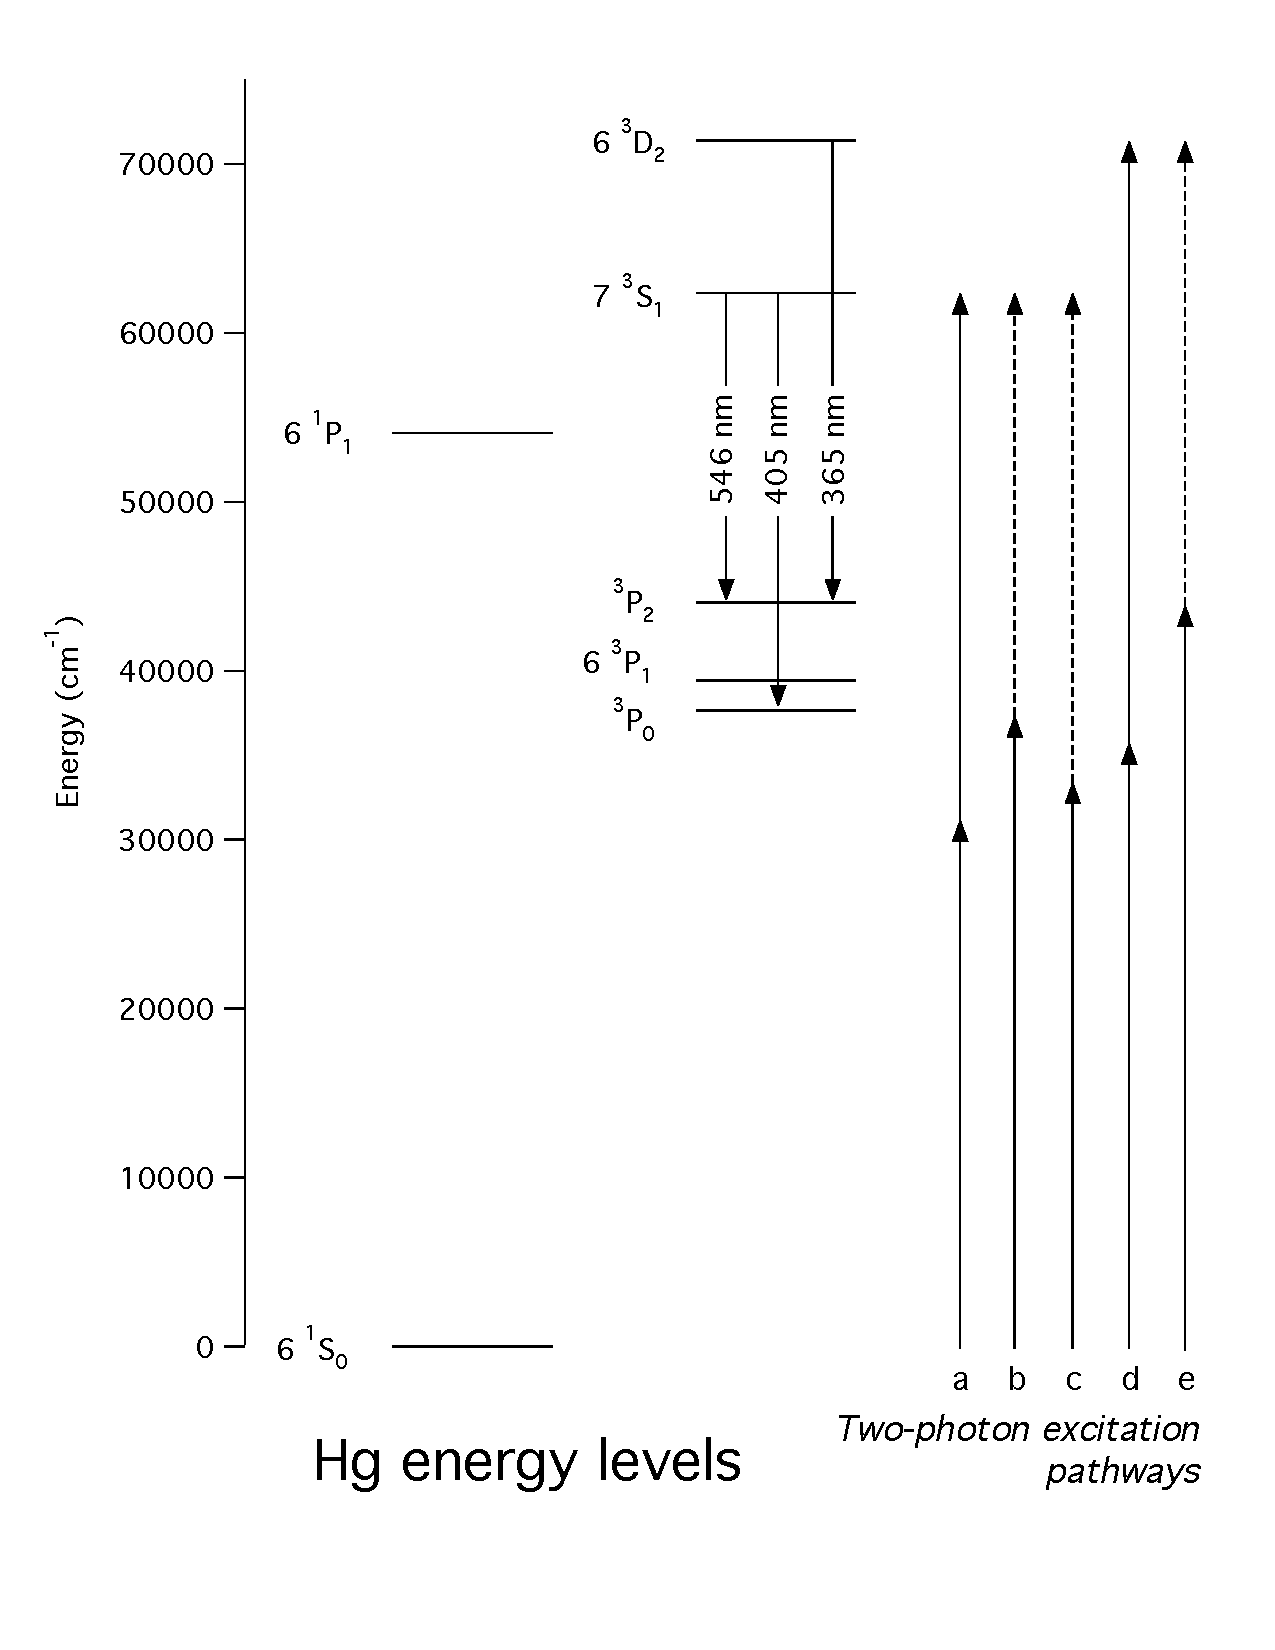
\includegraphics[height=8in,trim=4mm 0 0 0]{Hg-opticalpumpingschemes.pdf}
\end{figure}

\begin{figure}
  \caption{Calculated two-photon transition probabilities for the five
    possible excitation schemes discussed in the text.  Total
    probabilities depend on the square of laser intensity; quantities
    given in the figure are in units of s$^{-1}$W$^{-2}$.  The
    calculation indicates that the one color TPA to Hg*($7 \; ^3S_1$)
    is exactly zero.  Transition probabilities for excitation to the
    Hg*($6 \; ^3D_2$) level are two order of magnitude higher than the
    weakly allowed two color, two-photon transition probabilities to
    Hg*($7 \; ^3S_1$).}
  \label{fig:tpa-prob}
  \centering
  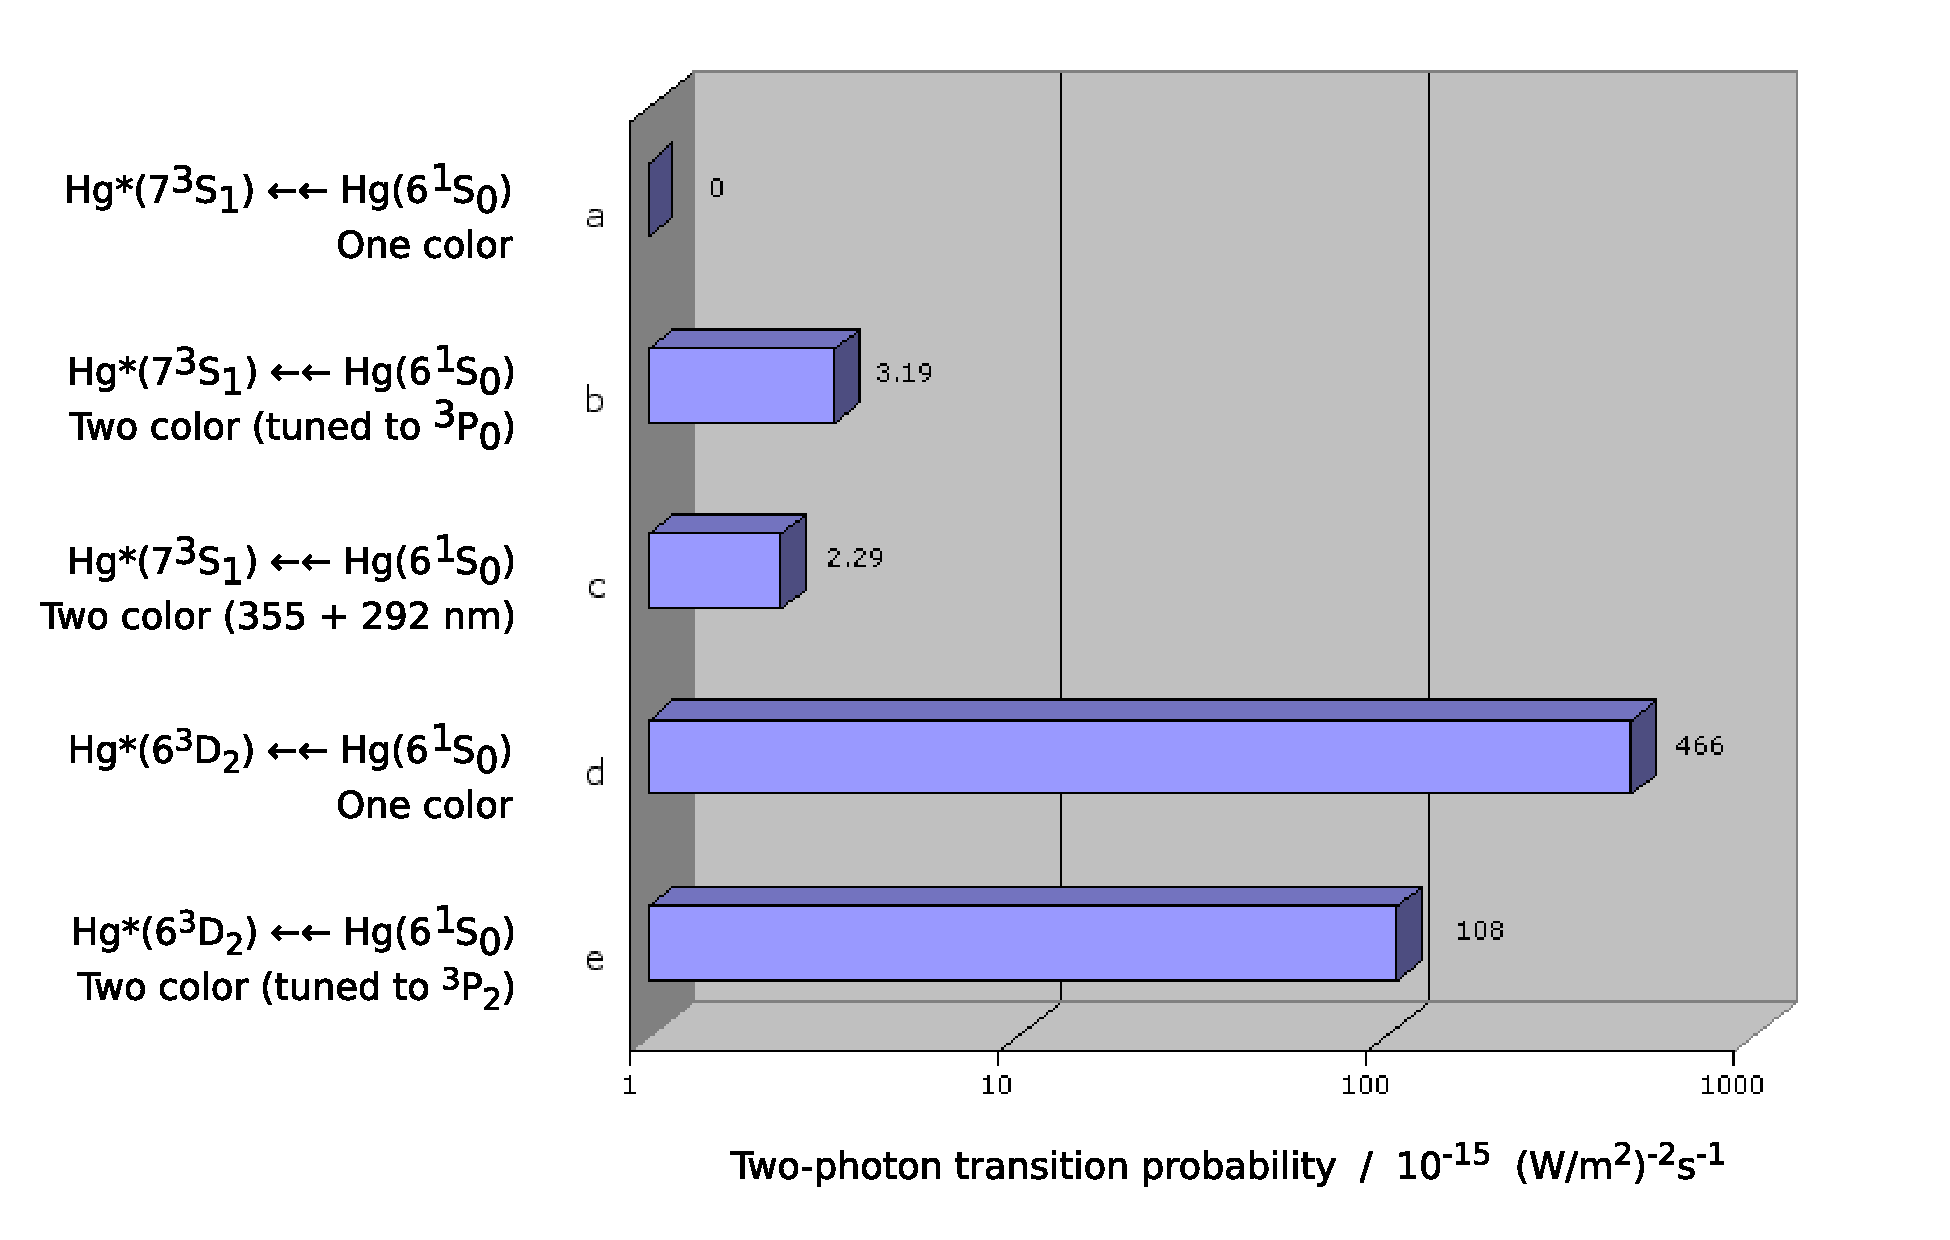
\includegraphics[width=7in,angle=90]{tpt-probs.pdf}
\end{figure}

The calculated transition probabilites for each scheme are displayed
in Figure \ref{fig:tpa-prob}.  The one color, two-photon transition to
the $6 \; ^3D_2$ level, item (d), has the greatest transition
probability among all the two-photon schemes considered.  The
two-color transition to $6 \; ^3D_2$, item (e), is slightly weaker.
The two color two-photon excitation schemes to the $7 \; ^3S_1$ level,
items (b) and (c), are an order of magnitude weaker yet, and the
one-color two-photon excitation to $7 \; ^3S_1$, item (a), is
forbidden entirely.

The Hg*($7 \; ^3S_1$) $\leftarrow\leftarrow$ Hg($6 \; ^1S_0$)
two-photon transition is rigorously forbidden according to the
selection rule $J=1 \nleftrightarrow J=0$ for photons of equal
frequency and any relative polarization \cite{bonin84}.  The rule may
be rationalized by considering the interference between quantum
mechanical pathways leading from the initial to final state
\cite{bonin84, grynberg77}.  Figure \ref{fig:hg-forbidden} shows
several of the possible pathways, as well as their relative phases
according to Formula \ref{eq:tpa-prob}.  It can be seen that the
amplitudes for the two different orderings of photon absorption are
equal and opposite.  In fact, experimental verification of this
two-photon selection rule is proposed as a test for the validity of
some fundamental principles of quantum field theory \cite{hilborn02}.

\begin{figure}
  \caption{Diagram of the interfering excitation pathways in $J'=1
    \leftarrow J''=0$ two-photon transitions with equal frequency
    photons.  Any choice of polarization results in equal but opposite
    amplitudes and for the two possible photon orderings. Since
    amplitudes for both orderings of the photons are summed and then
    squared in Equation \ref{eq:tpa-prob}, two-photon transition
    probability is rigorously cancelled by interference between
    alternate excitation pathways. The figure on the left illustrates
    the pathways for left and right circularly polarized photons,
    while the figure to the right illustrates the pathways for
    $z$-polarized and right circularly polarized photons.  The phase
    of each transition amplitude is indicated by either a solid or
    dashed arrow.}
  \label{fig:hg-forbidden}
  \centering
  \vspace{5mm}
  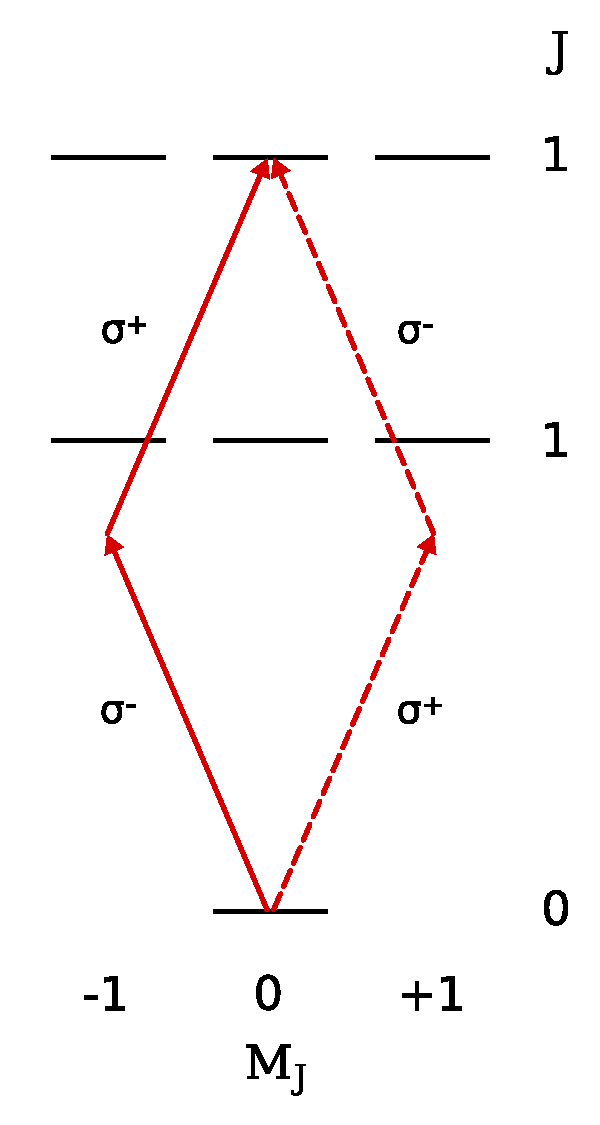
\includegraphics[width=2.7in]{hg-forbidden-samepol.pdf}
  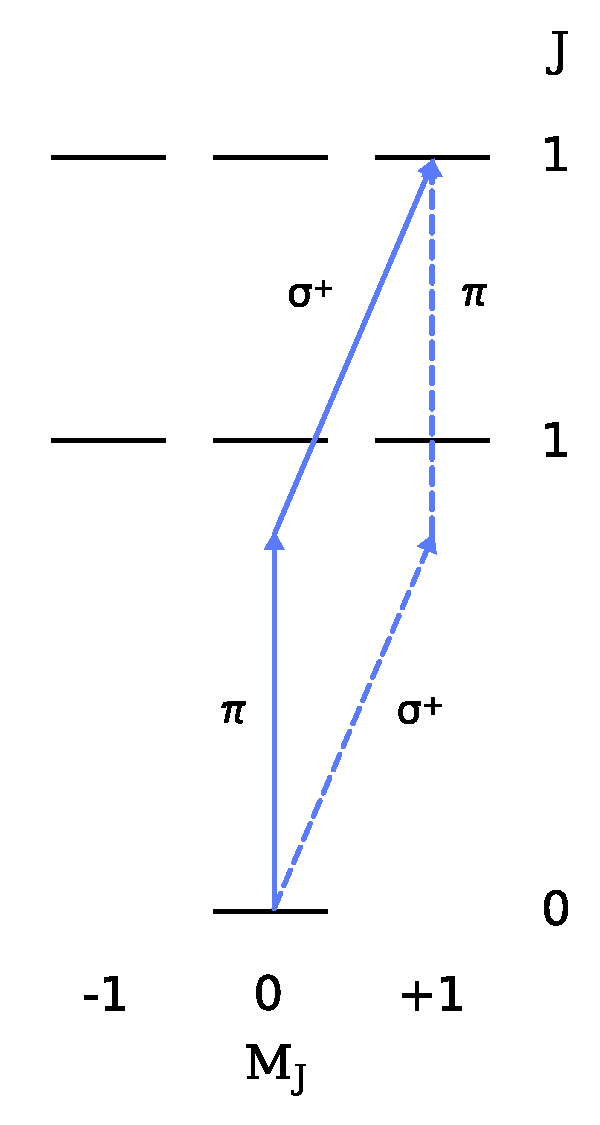
\includegraphics[width=2.7in]{hg-forbidden-perppol.pdf}
\end{figure}

\section{Theory: A collision model for electronic excitation transfer}

We base or mercury model on a collisional energy transfer model
originally developed for the Xe + \ce{N2} system by Ottinger and
Aquilanti \cite{aquilanti90, aquilanti94}.

Metastable xenon in the $^3P_2$ state transfers selectively into the
v'=5 level of \ce{N2}*($B\; ^3\Pi_g$) \cite{krumpelmann87,
  krumpelmann88, ottinger95b, aardema94}.  The process proceeds with
an absolute cross section of 6.5 $\AA$ \cite{bohle89}.

The angular momentum coupling rules for $P$-state atom collisions are
detailed by Aquilanti and coworkers \cite{aquilanti80a, aquilanti80b}.
The formalism is based on the idea of collisional Hund's cases,
explained by Nikitin and Zare \cite{nikitin94}.

The interaction potentials for $6 \; ^3P_0$ and $6 \; ^3P_2$ may be
estimated from those of the $6 \; ^3P_1$ state.  Having potential
surfaces in the collisional Hund's case (c) basis, the isotropic and
anisotropic parts of the interaction potentials may be determined
\cite{aquilanti89}.

Interest in the process of mercury photosensitization has led to the
study of the reaction of Hg $6 \; ^3P_1$ with many species
\cite{duval91, ohmori96}.  The parameters of 

\begin{figure}
  \caption{Potential energy curves and vibrational levels of the three
    ``lowest'' energy triplet electronic states of nitrogen, \ce{N2}.
    The $A$ state is metastable, with a fluorescence lifetime in the
    hundreds of microseconds.  Molecules in the $W$ state decay slowly
    to the near-degenerate $B$ electronic state via the emission of IR
    fluorescence.  The fluorescence lifetime for $B \rightarrow A$
    emission is several \microsec. It is this 400$-$500 nm
    fluorescence that we measure to observe the preparation of
    metastable \ce{N2}.  Also shown in the figure is the energy of the
    xenon $^3P_2$ state, which is known to populate the v'=5 level of
    the nitrogen $B$ state in gas-phase collisions
    \cite{krumpelmann87}.  Less is known about electronic energy
    transfer from Xe into the $W$ state of nitrogen, however, the
    ultimate decay route is unchanged in any case.  The figure is
    adapted from Reference \cite{krumpelmann-thesis}.}
  \label{fig:n2curves}
  \centering
  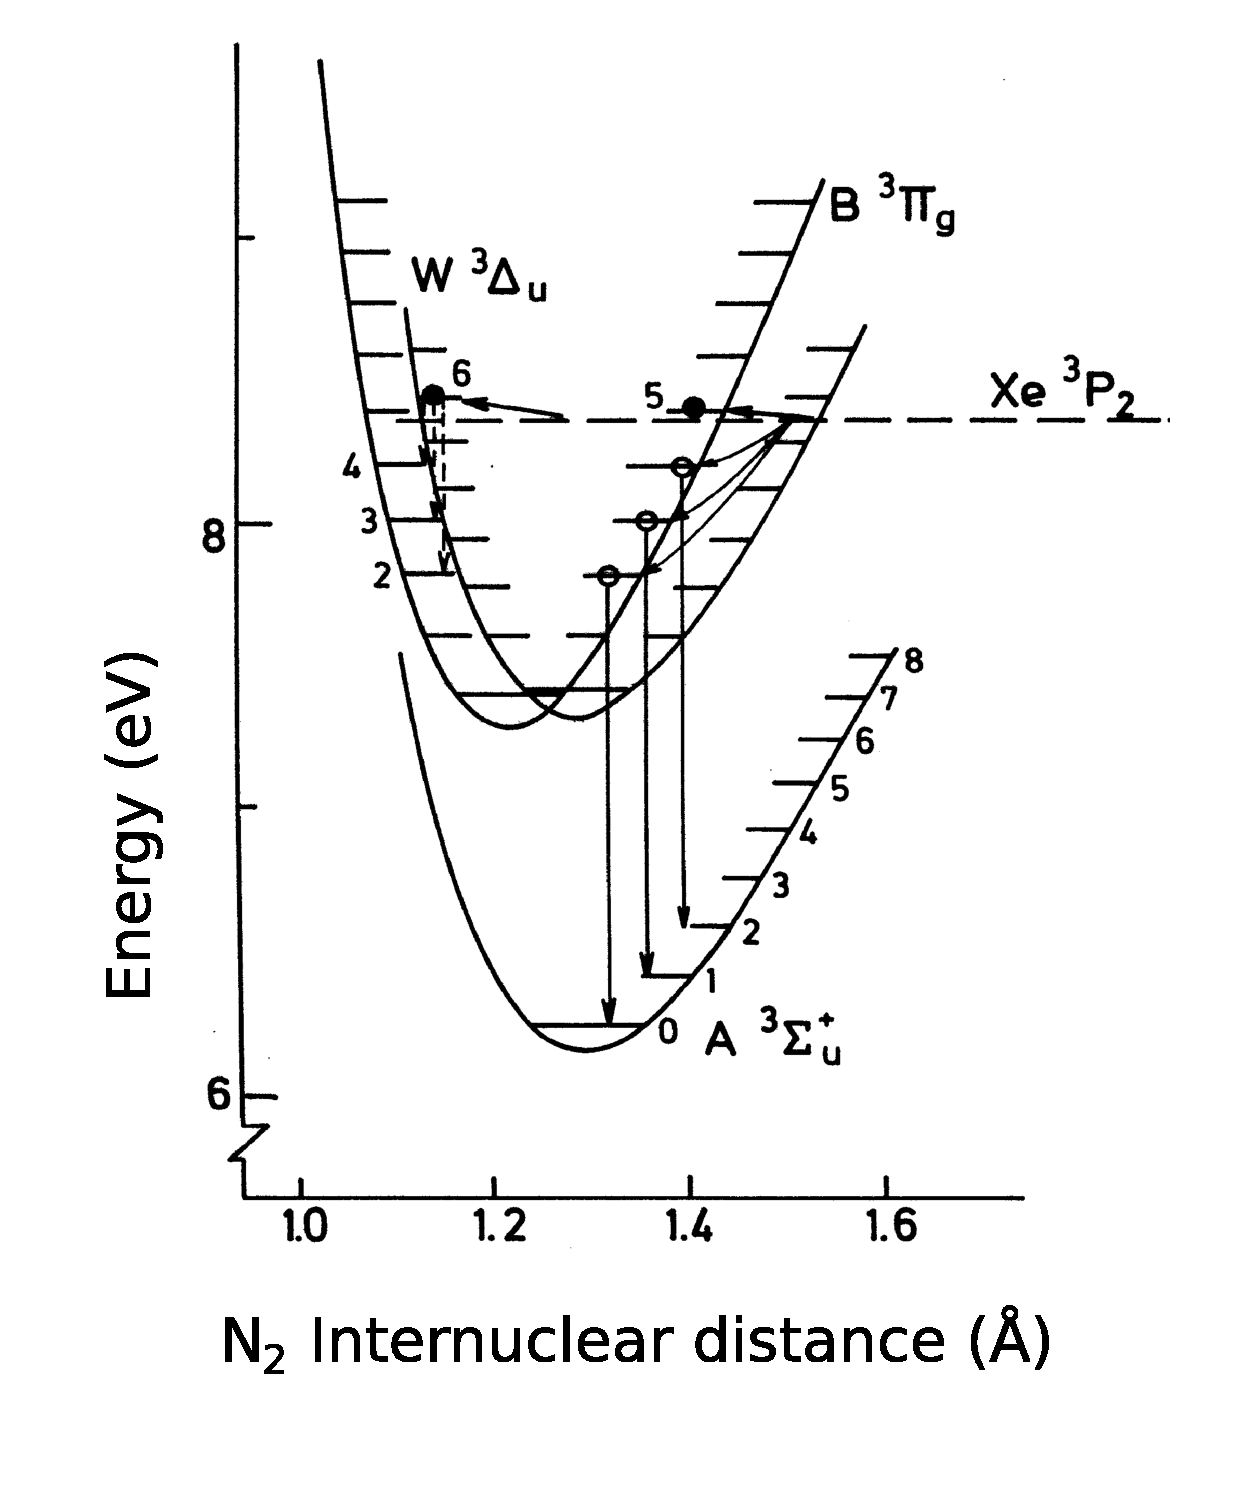
\includegraphics[width=5in]{n2curves.pdf}
\end{figure}

\section{Experiments: \ce{Xe}* + \ce{N2}}

We investigate the \ce{Xe}* + \ce{N2} system as a precursor to our
experiments with mercury and acetylene.  Besides its status as a
well-studied reaction and the foundation of our adopted curve crossing
model, the xenon-nitrogen system has the advantage of high excitation
energies.  The lowest excited state of xenon, $^3P_2$, lies 8.3 eV
above the ground state \cite{saloman04}.  The lowest triplet state of
nitrogen, $A \; ^3\Sigma_u^+$, while far below Xe*($^3P_2$), lies 6.2
eV above the ground state \cite{lofthus77}.  (Triplet electronic
states of nitrogen are labeled with uppercase letters for historical
reasons.)  The energies of Xe*($^3P_2$) and \ce{N2}($A \;
^3\Sigma_u^+$) far exceed the work function of gold, and both species
are extremely metastable \cite{mishra01, lofthus77}.

Two-photon excitation of xenon atoms is fairly common among atomic
physicists \cite{alekseev96}.  To populate Xe*($^3P_2$), we use the
one color, two-photon excitation to the $^3D_2$ state.  The $^3D_2$
state decays spontaneously to $^3P_1$ and $^3P_2$ with a branching
ratio of 1:2 \cite{cabrera81}.  The two-photon transition probability
for Xe*($^3D_2$) $\leftarrow\leftarrow$ Xe($^1S_0$) was calculated in
the same manner as the Hg transitions.  A total probability of
3.35$\times$10$^{-14}$ (W/m$^2$)$^{-2}$s$^{-1}$ is obtained for the
one color TPA.  The magnitude of the xenon two-photon transition
probability is approximately 1/10th that of the analagous transition
in Hg.

The LIF spectrum of the xenon $^3D_2$ $\leftarrow\leftarrow$ $^1S_0$
two-photon transition was recorded first in a static cell (Figure
\ref{fig:xe3d2-cell}) and then in a molecular beam (Figure
\ref{fig:xe-beam}).  The $^3D_2$ $\rightarrow$ $^3P_2$ fluorescence
emission at 823 nm was passed through a colored glass filter and
collected by a Hamamatsu R375 photomultiplier tube.  Emission to the
$^3P_1$ state at 895 nm was outside the wavelength response range of
the photomultiplier.  The fluorescence decay, plotted in the bottom of
Figure \ref{fig:xe-beam}, is consistent with the fluorescence lifetime
of $\tau = 28$ ns reported in the literature \cite{cabrera81}.

\begin{figure}
  \caption{Laser-Induced Fluorescence (LIF) spectrum of the one color,
    two photon transition \ce{Xe} $^3D_2 \leftarrow \leftarrow
    ^1S_0$, recorded under static cell conditions.  The LIF signal
    results from spontaneous emission to the metastable $^3P_2$
    state at 823 nm.}
  \label{fig:xe3d2-cell}
  \centering
  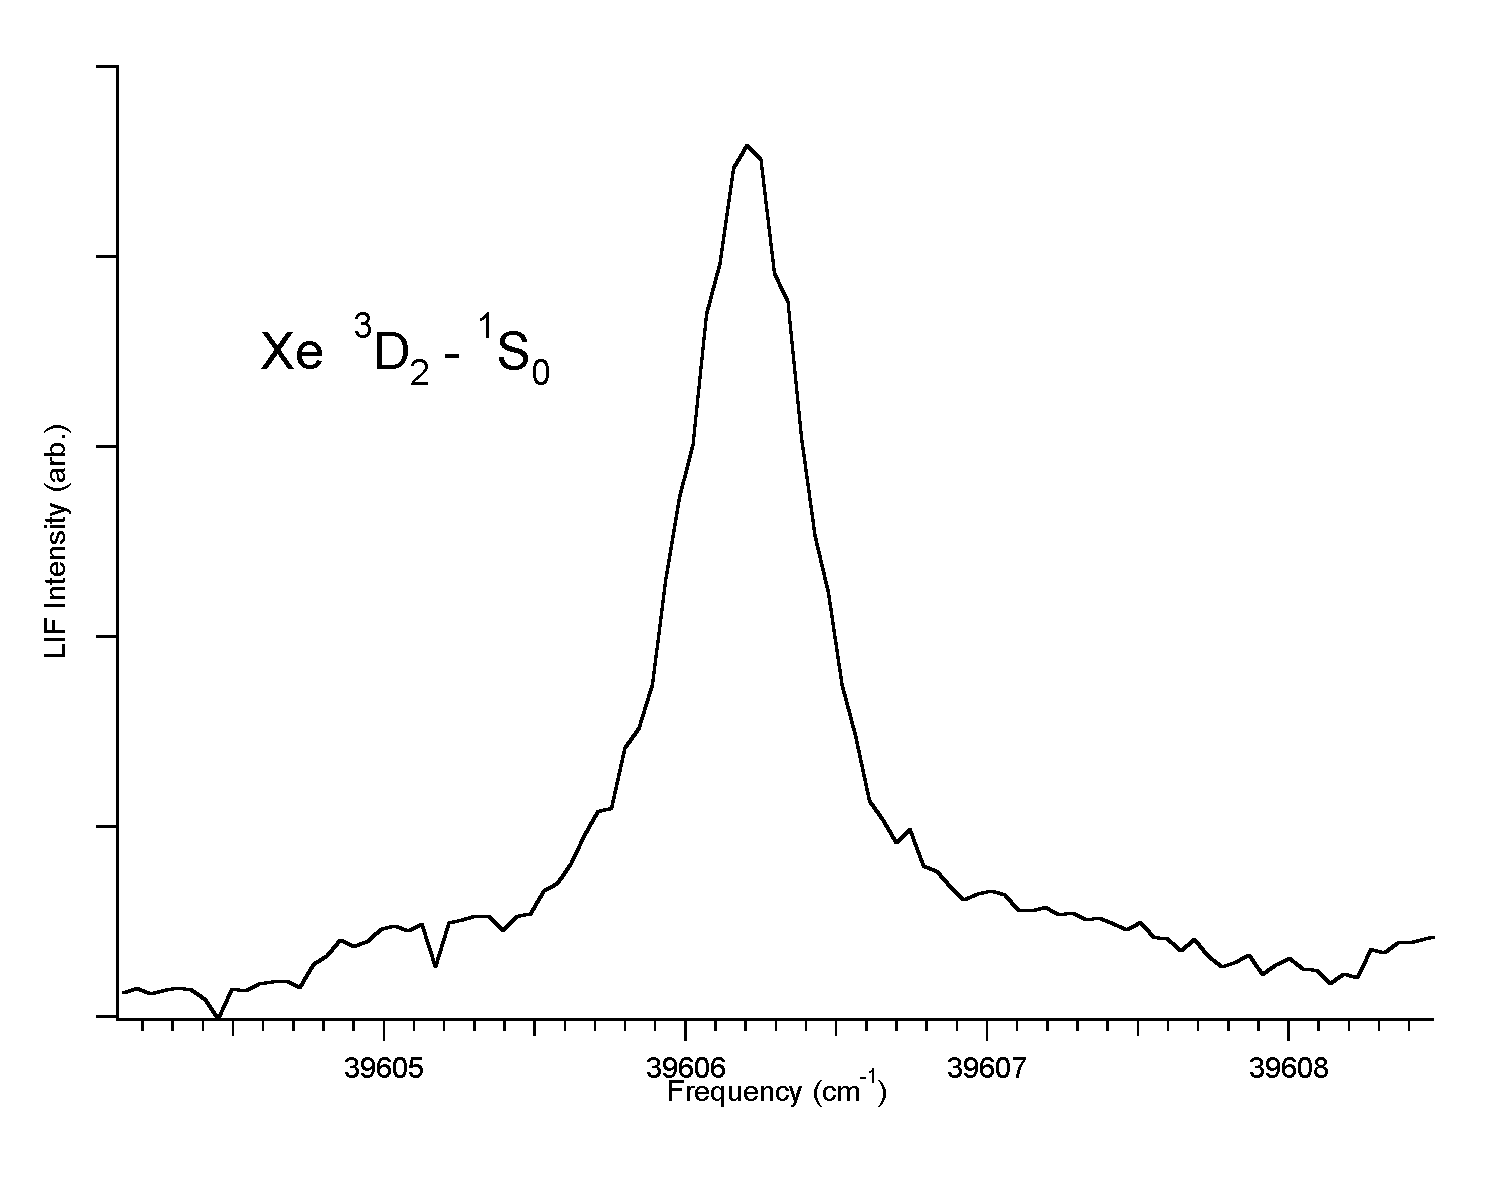
\includegraphics[width=6in]{Xe3D2-cell.pdf}
\end{figure}

\begin{figure}
  \caption{(Top) Laser-Induced Fluorescence (LIF) spectrum of the one
    color, two photon transition \ce{Xe} $^3D_2 \leftarrow \leftarrow
    ^1S_0$, recorded in a supersonic expansion.  (Bottom) Time
    dependence of \ce{Xe} $^3D_2 \rightarrow ^3P_2$ emission (solid
    trace), compared to a magnified signal resulting from scattered
    laser light (dashed trace). The fluorescence signal results from
    spontaneous emission to the metastable $^3P_2$ state at 823 nm
    ($\tau = 28$ ns).  \TODO{Change top plot to LIF intensity.}}
  \label{fig:xe-beam}
  \centering
  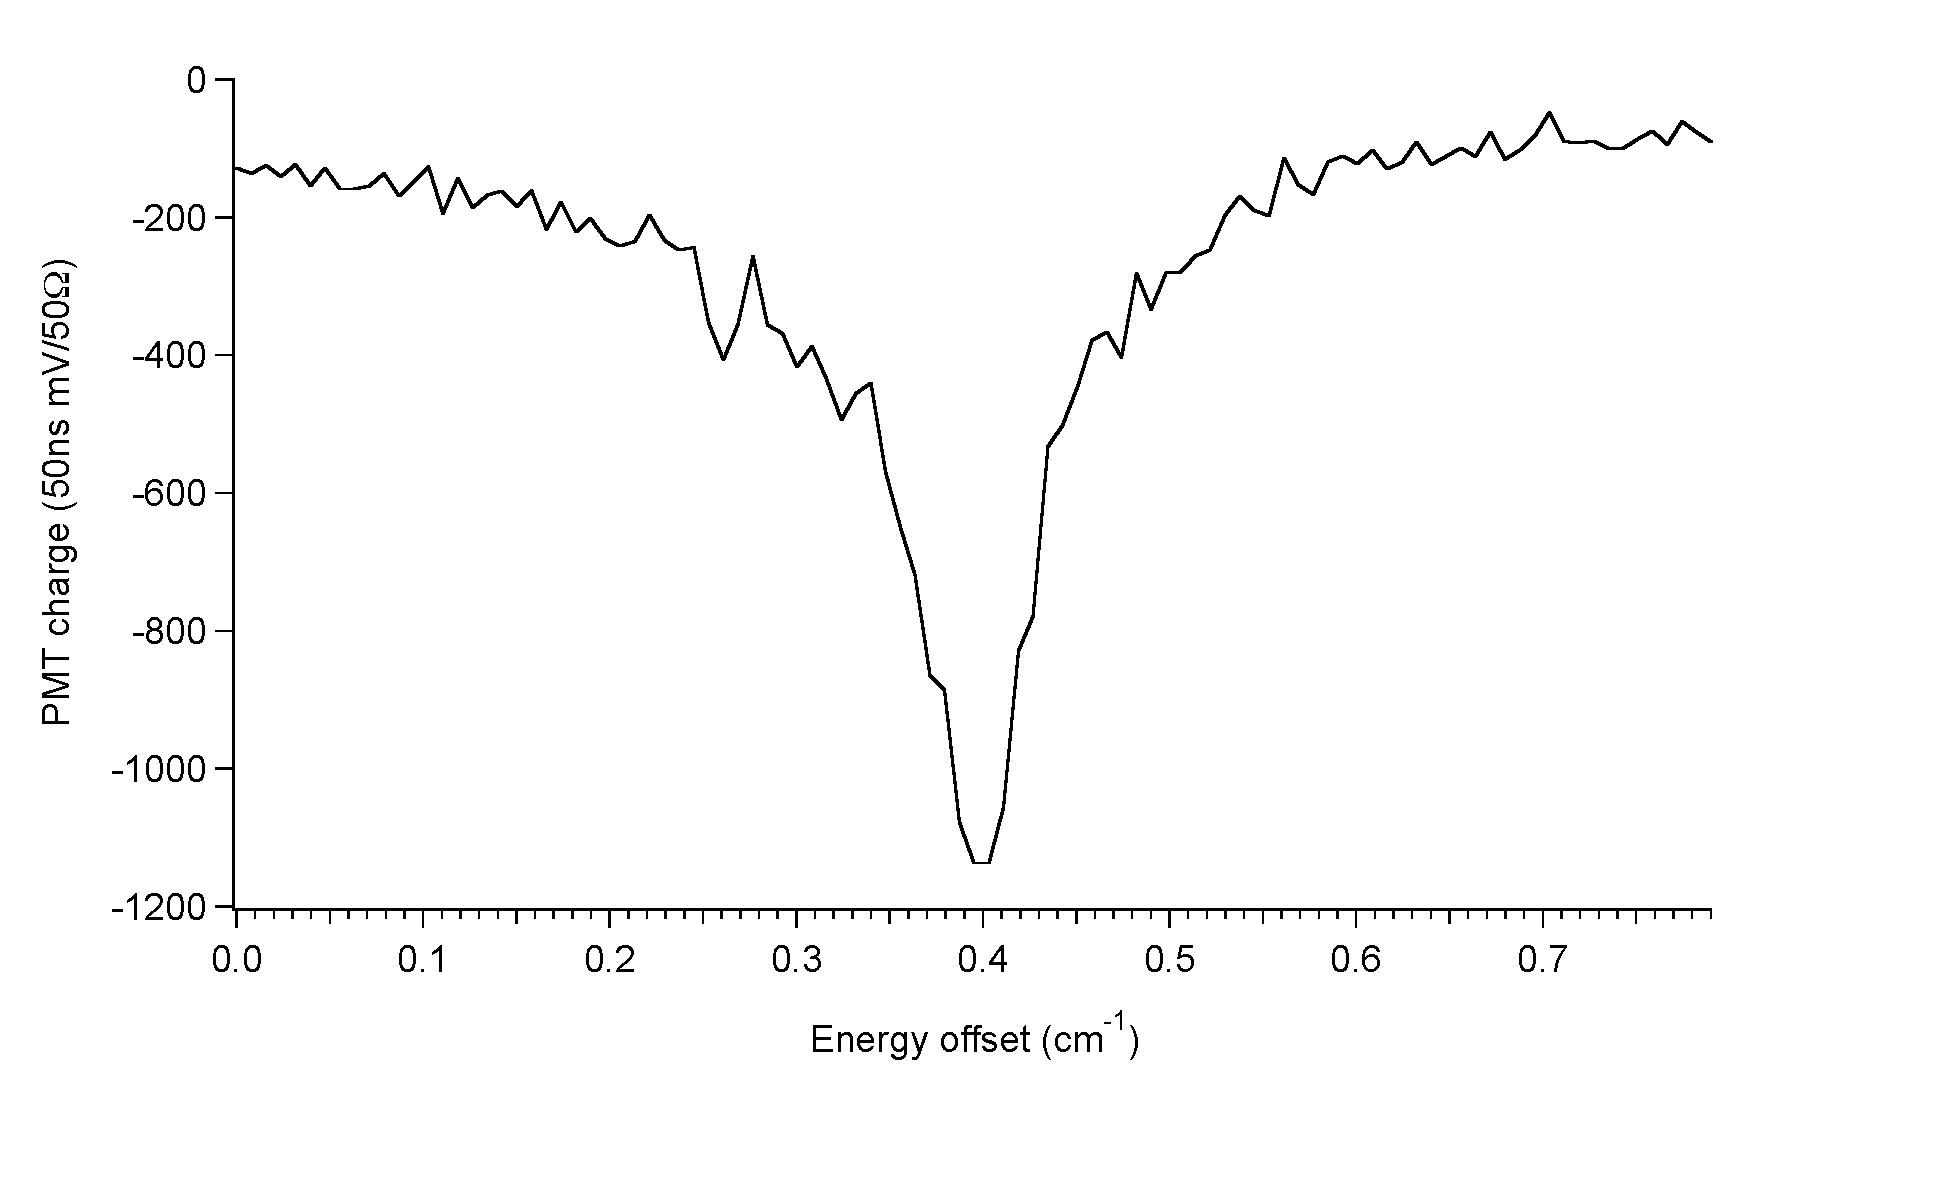
\includegraphics[width=6in]{Xe-beamlif-060406.pdf}
  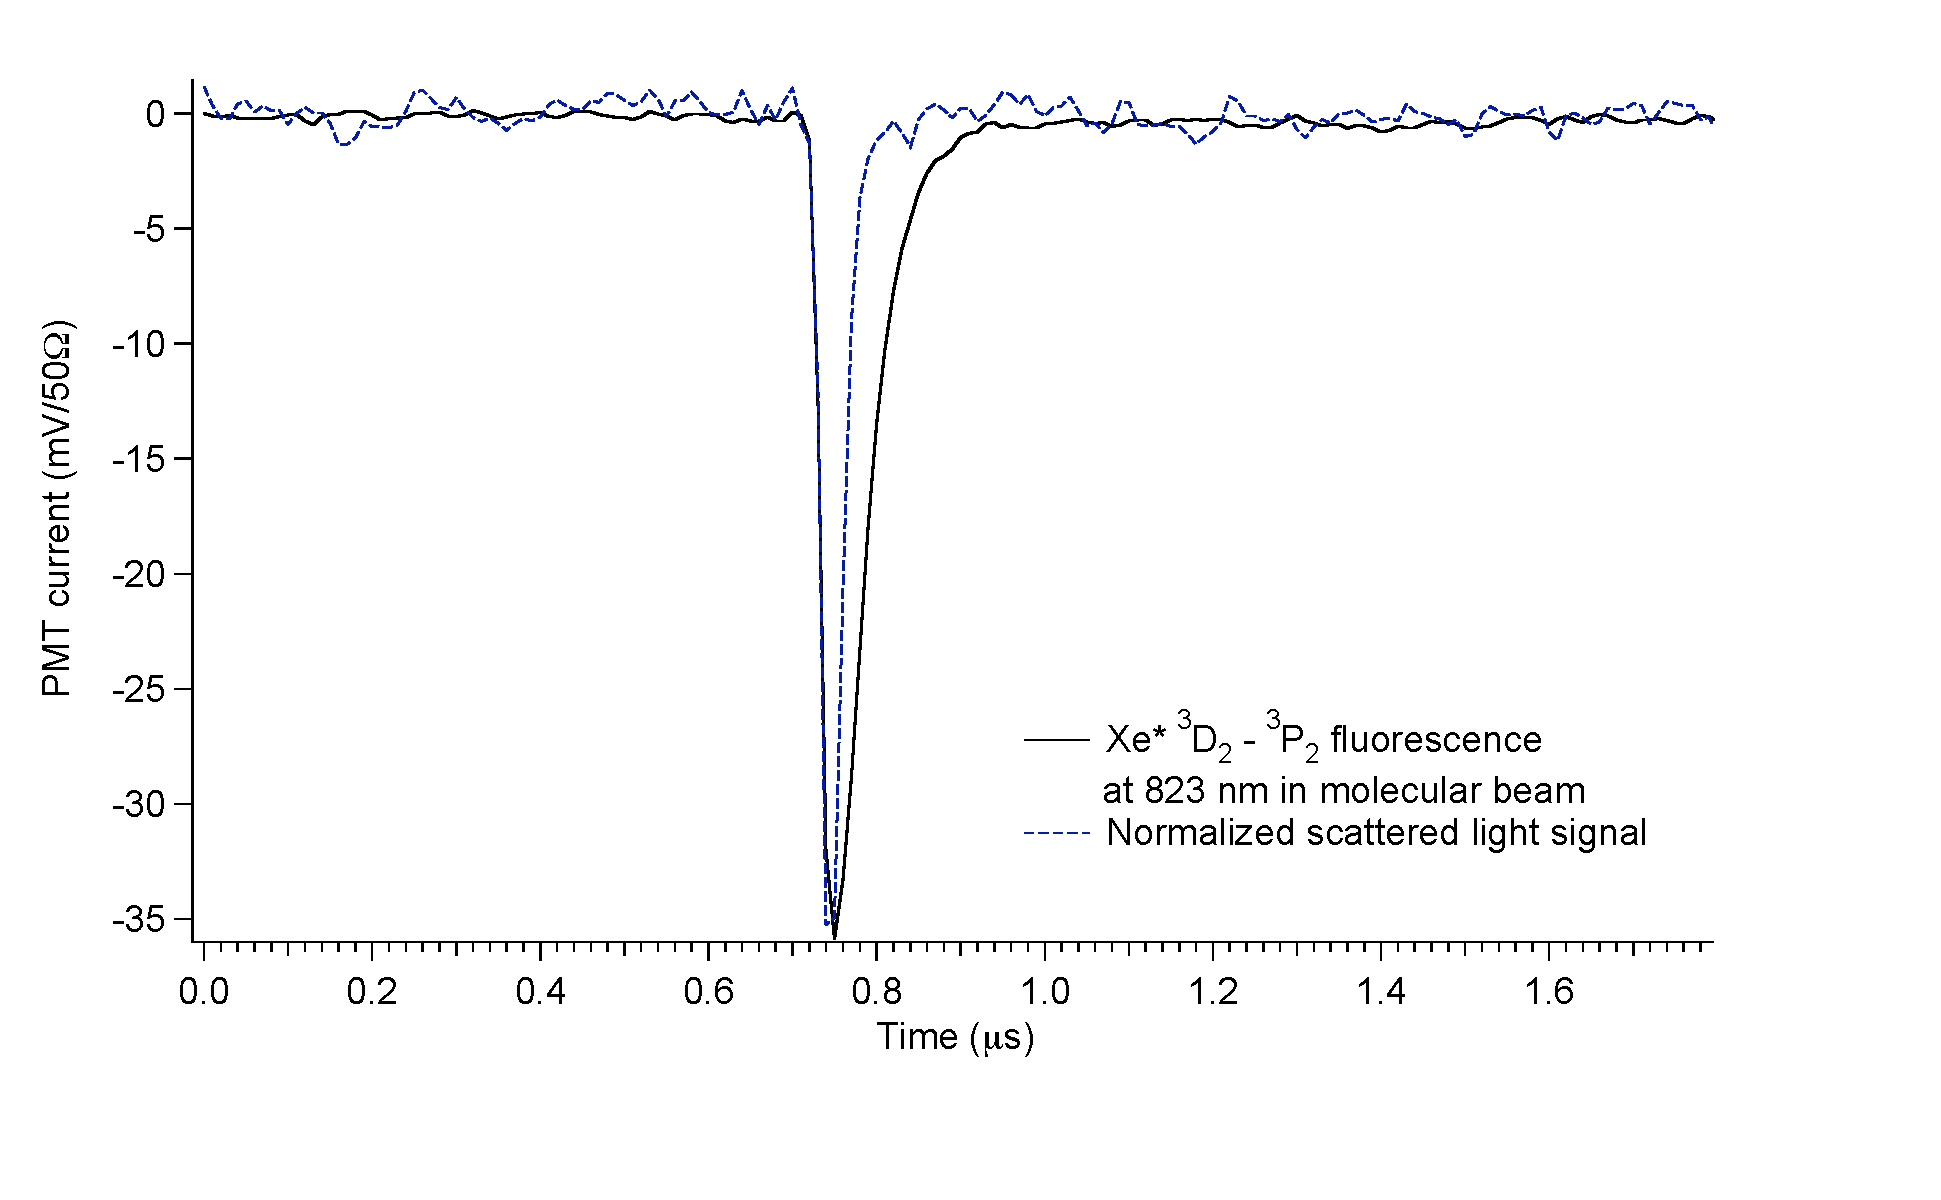
\includegraphics[width=6in]{Xe-beamtrc-060406.pdf}
\end{figure}

Electronic energy transfer to nitrogen molecules was measured first
under static cell conditions.  The excitation chamber of the SEELEM
apparatus was sealed and filled with 210 mTorr of a 50:50 Xe/\ce{N2}
gas mixture.  The laser was held fixed on the \ce{Xe} $^3D_2
\leftarrow \leftarrow ^1S_0$ two-photon transition.  Collision-induced
\ce{N2} $B \rightarrow A$ emission in the visible region of the
spectrum is plotted in Figure \ref{fig:xen2-firstlight}.  Our
observation is consistent with the reported fluorescence lifetime of
\ce{N2} $B \rightarrow A$ emission, which is on the order of 10
\microsec.

\begin{figure}
  \caption{Time dependence of \ce{N2} $B \rightarrow A$ emission,
    induced by collisions with metastable Xe* ($^3P_2$).  The
    excitation chamber of the SEELEM apparatus was sealed and filled
    with a 50:50 mixture of Xe and \ce{N2}, to a total pressure of 210
    mTorr.  Metastable Xe*($^3P_2$) was populated by spontaneous
    emission, following the $6\;^3D_2 \leftarrow \leftarrow 6\;^1S_0$
    two-photon transition.}
  \label{fig:xen2-firstlight}
  \vspace{1cm}
  \centering
  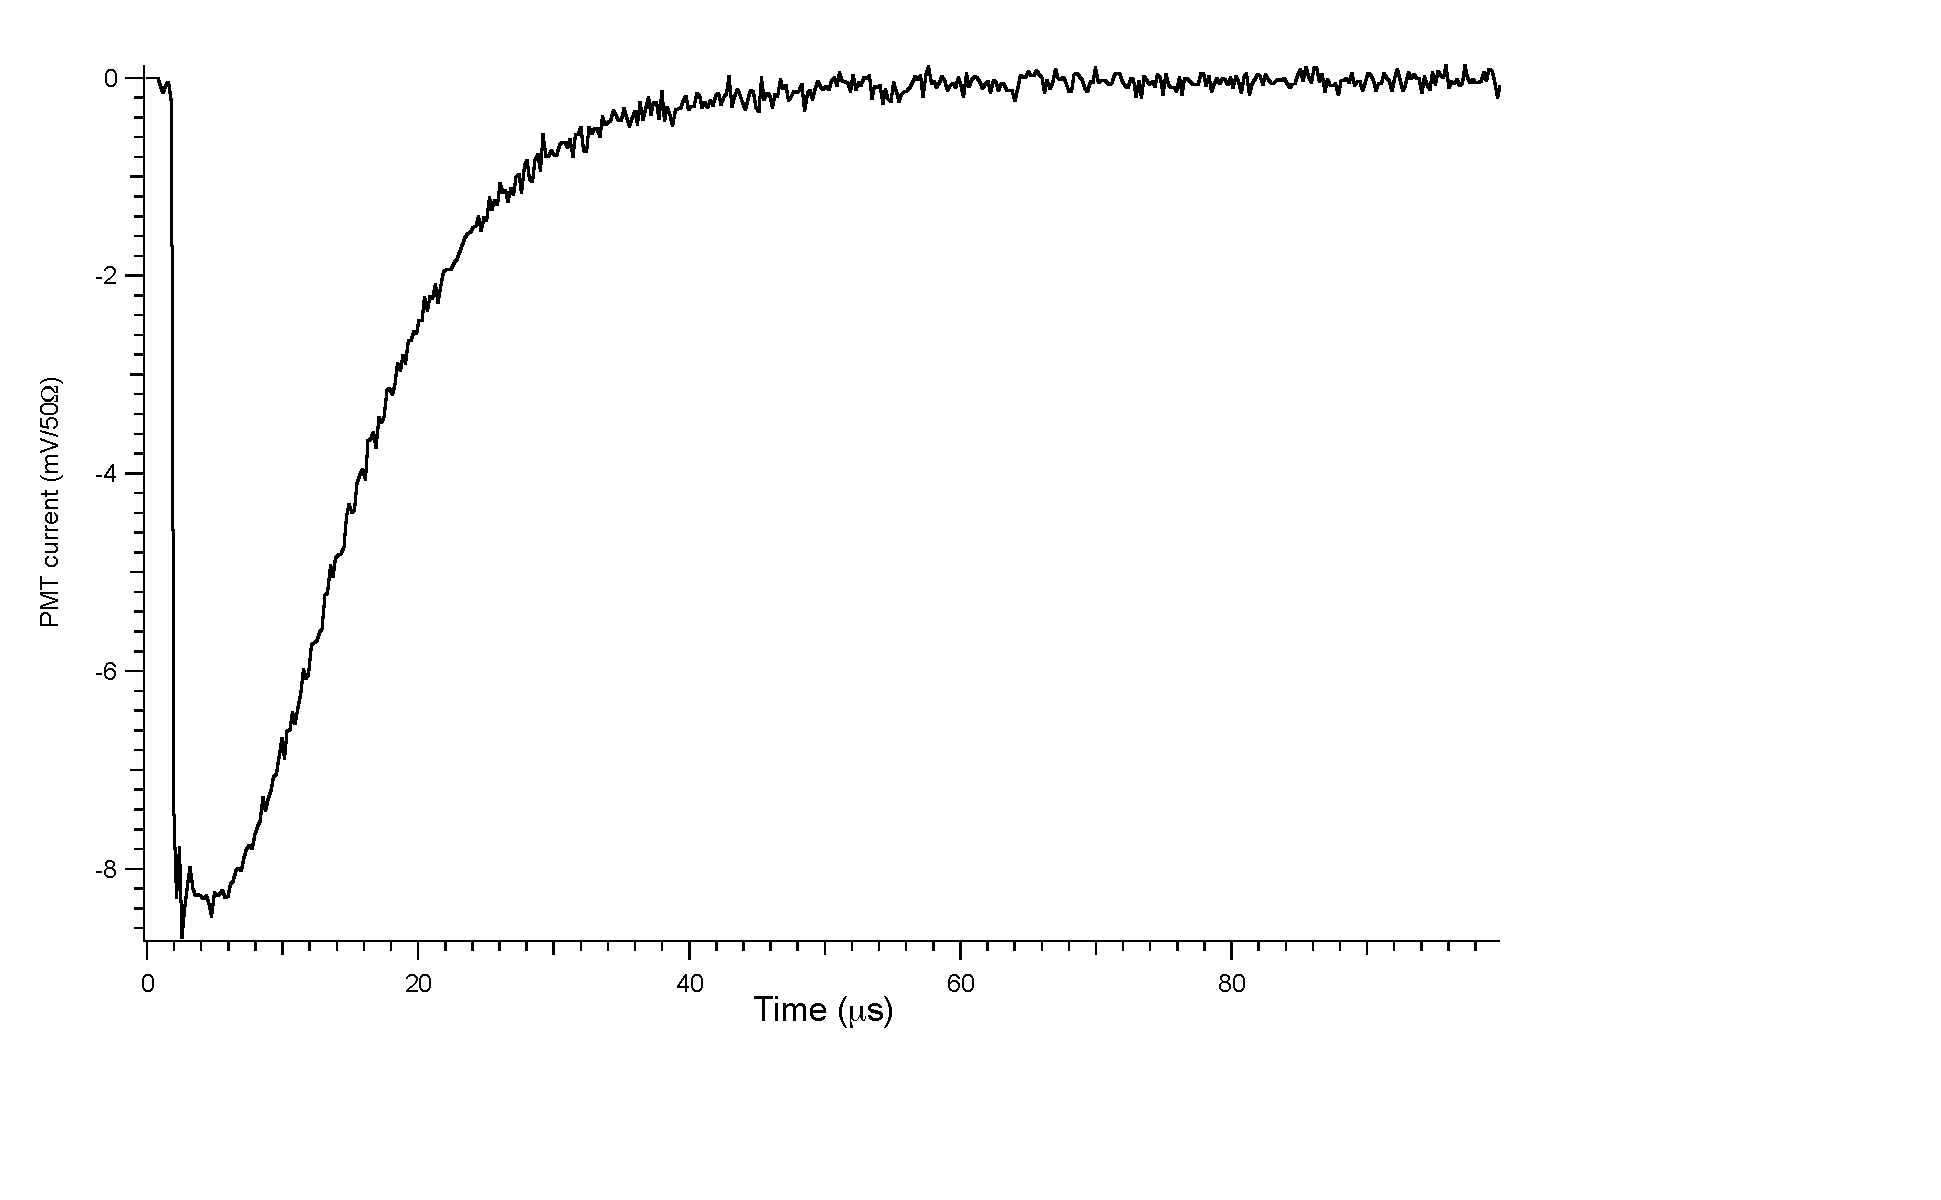
\includegraphics[width=7in]{XeN2-firstlight.pdf}
  \vspace{2in}
\end{figure}

To carry out the excitation in the early stages of a supersonic
expansion, a short nozzle extension was constructed.  The extension
piece consisted of a cylinder of stainless steel, 2 cm in length, with
a 1 mm diameter bore.  The piece was tapered at the end to maximize
the exposure of the orifice to laser radiation.  The nozzle extension
allowed the laser radiation to intersect the free jet im the high
pressure region immediately in front of the nozzle orifice.

The two-photon excitation to Xe ($^3D_2$) was carried out in the
high-pressure region of a supersonic expansion with a 50:50 gas
mixture of Xe and \ce{N2}.  The time dependence of \ce{Xe} $6\;^3D_2
\rightarrow 6\;^3P_2$ and \ce{N2} $B \rightarrow A$ emission is
plotted in Figure \ref{fig:xen2-traces}.  Xenon fluorescence (823 nm,
$\tau=28$ ns) is emitted when the optically excited state decays
spontaneously to the metastable $6\;^3P_2$ state.  Nitrogen molecules
are electronically excited during the expansion process in collisions
with metastable xenon atoms.  Near-resonant vibrational levels of the
nitrogen $B$ state decay spontaneously to the metastable $A$ state
($\tau=20$ \microsec), accompanied by fluorescence in the visible
region of the spectrum.  Since the xenon and nitrogen fluorescence
decays occur on vastly different timescales, the time constant of the
oscilloscope must be adjusted separately for each measurement.

\begin{figure}
  \caption{Time dependence of \ce{Xe} $6\;^3D_2 \rightarrow 6\;^3P_2$
    (top plot) and \ce{N2} $B \rightarrow A$ (bottom plot) emission,
    following the two-photon excitation of Xe ($^3D_2$) in a
    supersonic expansion.  The xenon and nitrogen emission signals
    occur on vastly different timescales.  Xenon fluorescence (823 nm,
    $\tau=28$ ns) is emitted when the optically excited state decays
    spontaneously to the metastable $6\;^3P_2$ state.  Nitrogen
    molecules are electronically excited during the expansion process
    in collisions with metastable xenon atoms.  Near-resonant
    vibrational levels of the nitrogen $B$ state decay spontaneously
    to the metastable $A$ state ($\tau \approx 10$ \microsec),
    accompanied by fluorescence in the visible region of the
    spectrum. \TODO{Change voltage to current.}}
  \label{fig:xen2-traces}
  \centering
  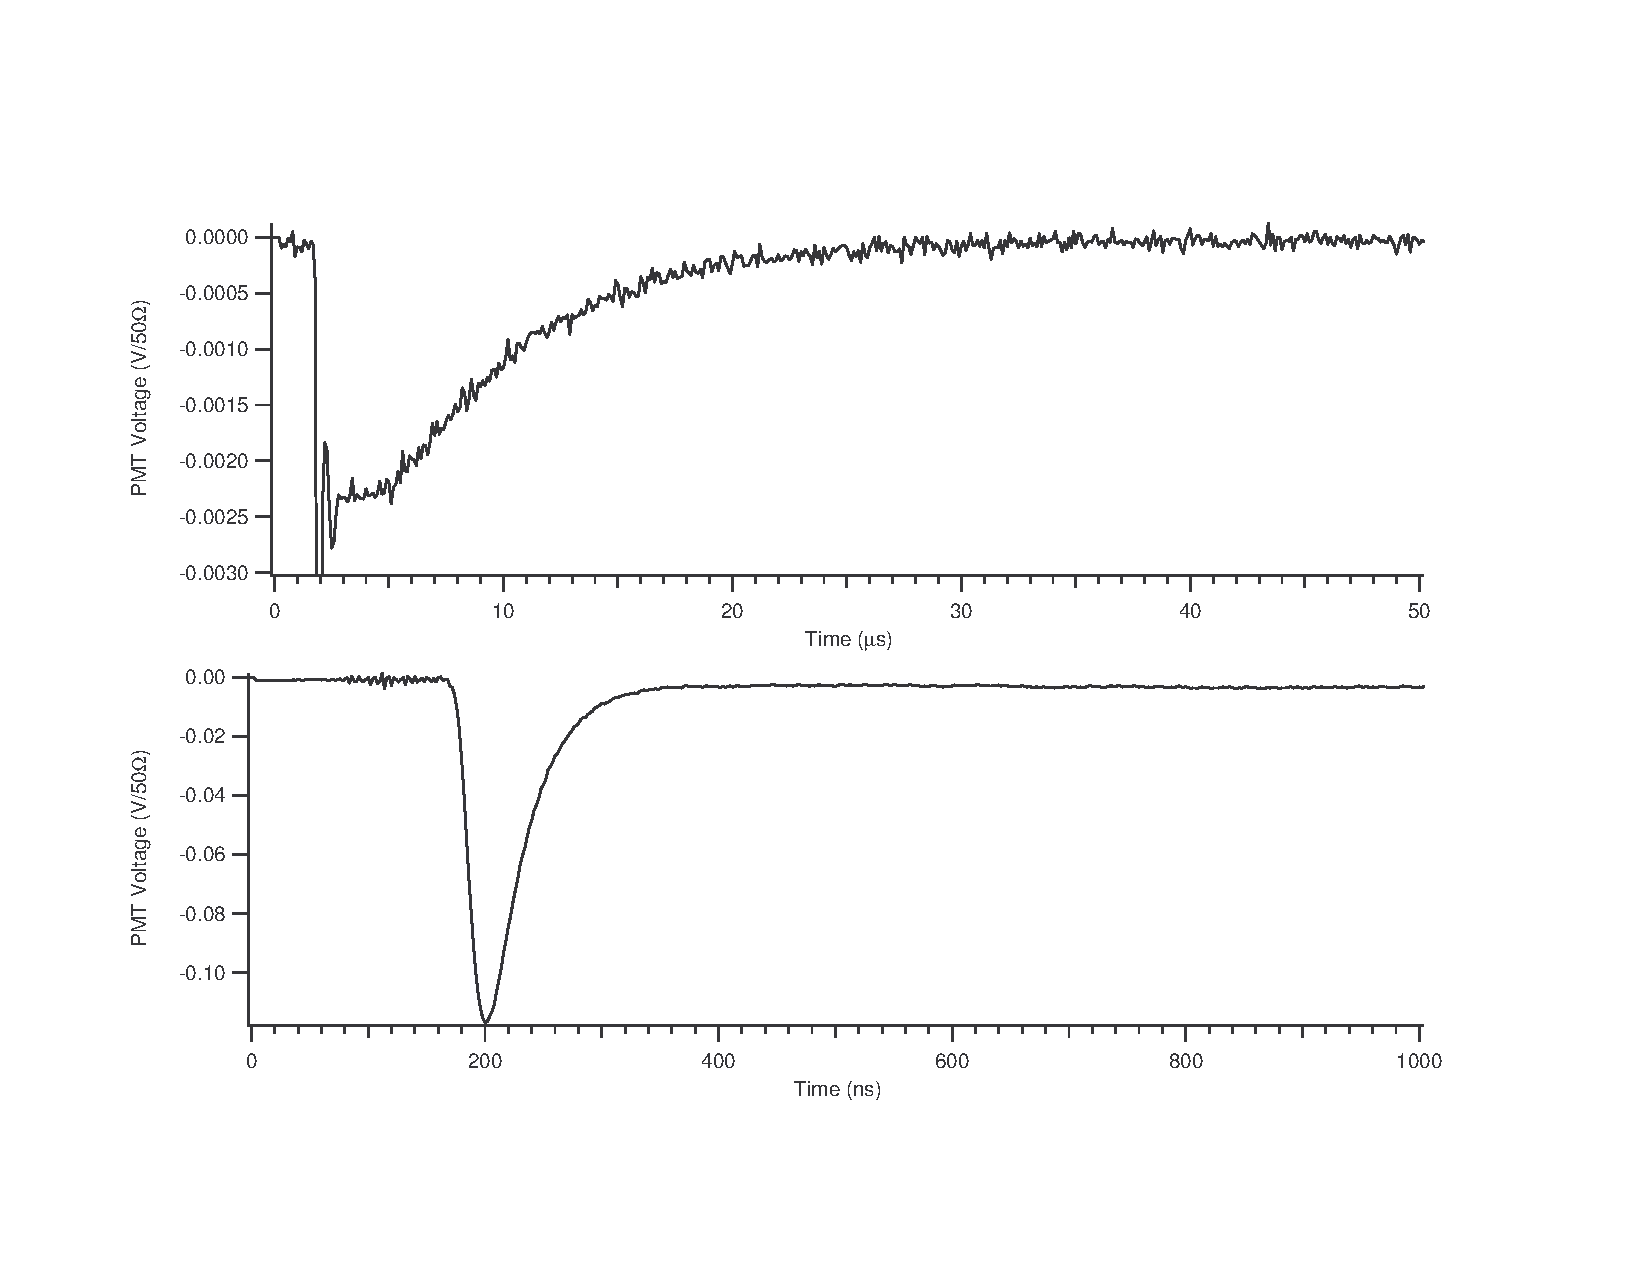
\includegraphics[width=7.7in,angle=90,trim=0 0 1in 1cm ]{XeN2-traces.pdf}
\end{figure}

\TODO{Xe seelem spectrum}

\TODO{Xe seelem tof}

\TODO{One N2 + Xe TOF spectrum}

% The TOF:SEELEM spectrum of metastable xenon is shown in Figure
% \ref{fig:xe-seelem}.  The limiting velocity of Xe in a molecular beam
% is approximately 308 m/s, which yields a flight time of .

% The average velocity of the pure xenon beam, based on
% the maximum of the TOF:SEELEM spectrum, is determined to be ??? m/s.
% Although this is slower than
% The velocity distribution in a molecular beam is
% \begin{equation}
%   P(v) = v^3 \exp 
%   \left [
%     -\frac{m(v-u(x))^2}{2RT(x)}
%   \right ],
% \end{equation}
% where $T(x)$ and $u(x)$ are the instantaneous temperature and flow
% velocity in the beam \cite{morse96}.









\section{Experiments: \ce{Hg}* + \ce{C2H2}}

The production of metastable molecules in a molecular beam using
collisional excitation by mercury is more of a challenge than xenon.
Firstly, the lowest metastable state of Hg, $^3P_2$, is too low in
energy to be detectable on gold.  Secondly, the only allowed
triplet-triplet transition in acetylene is in the infrared, and the
product of the transition $T_1$ is not detectable even on a
medium-work function metal such as Y.

Yet another challenge is generating the required number densities of
mercury in the pulsed nozzle.  The Jordan valve normally used for
SEELEM experiments may only be heated to 120\degrees\ C.  Another
nozzle design, capable of higher temperatures, was needed for our
experiments.  Heated continuous beam sources of mercury $6 \; ^3P_0$
are reported in the literature \cite{haberman75, obi83}.  Nitrogen
backing gas is first bubbled through a mercury oven before expanding
from a nozzle with an embedded resonance lamp.  However, we required a
pulsed design due to pump speed limitations.  

A new pulsed valve was designed by Wilton Virgo to meet our demands
for heated mercury.  The new valve is based on a pulsed valve used by
the Leutwyler research group in Bern, Switzerland.  The valve can be
heated to 250\degrees\ C, corresponding to a mercury vapor pressure of
??? Torr.  A diagram of the ``Bern Valve'' is shown in Figure
\ref{fig:bern-diagram}.

\begin{figure}
  \caption{Diagram of the heated pulsed valve developed for
    experiments with mercury.  The ``Bern Valve'' can be safely heated
    to 250\degrees\ C.  A small vial of mercury is housed in the
    heated region on the right of the diagram, close to the nozzle
    orifice (far right).}
  \label{fig:bern-diagram}
  \centering
  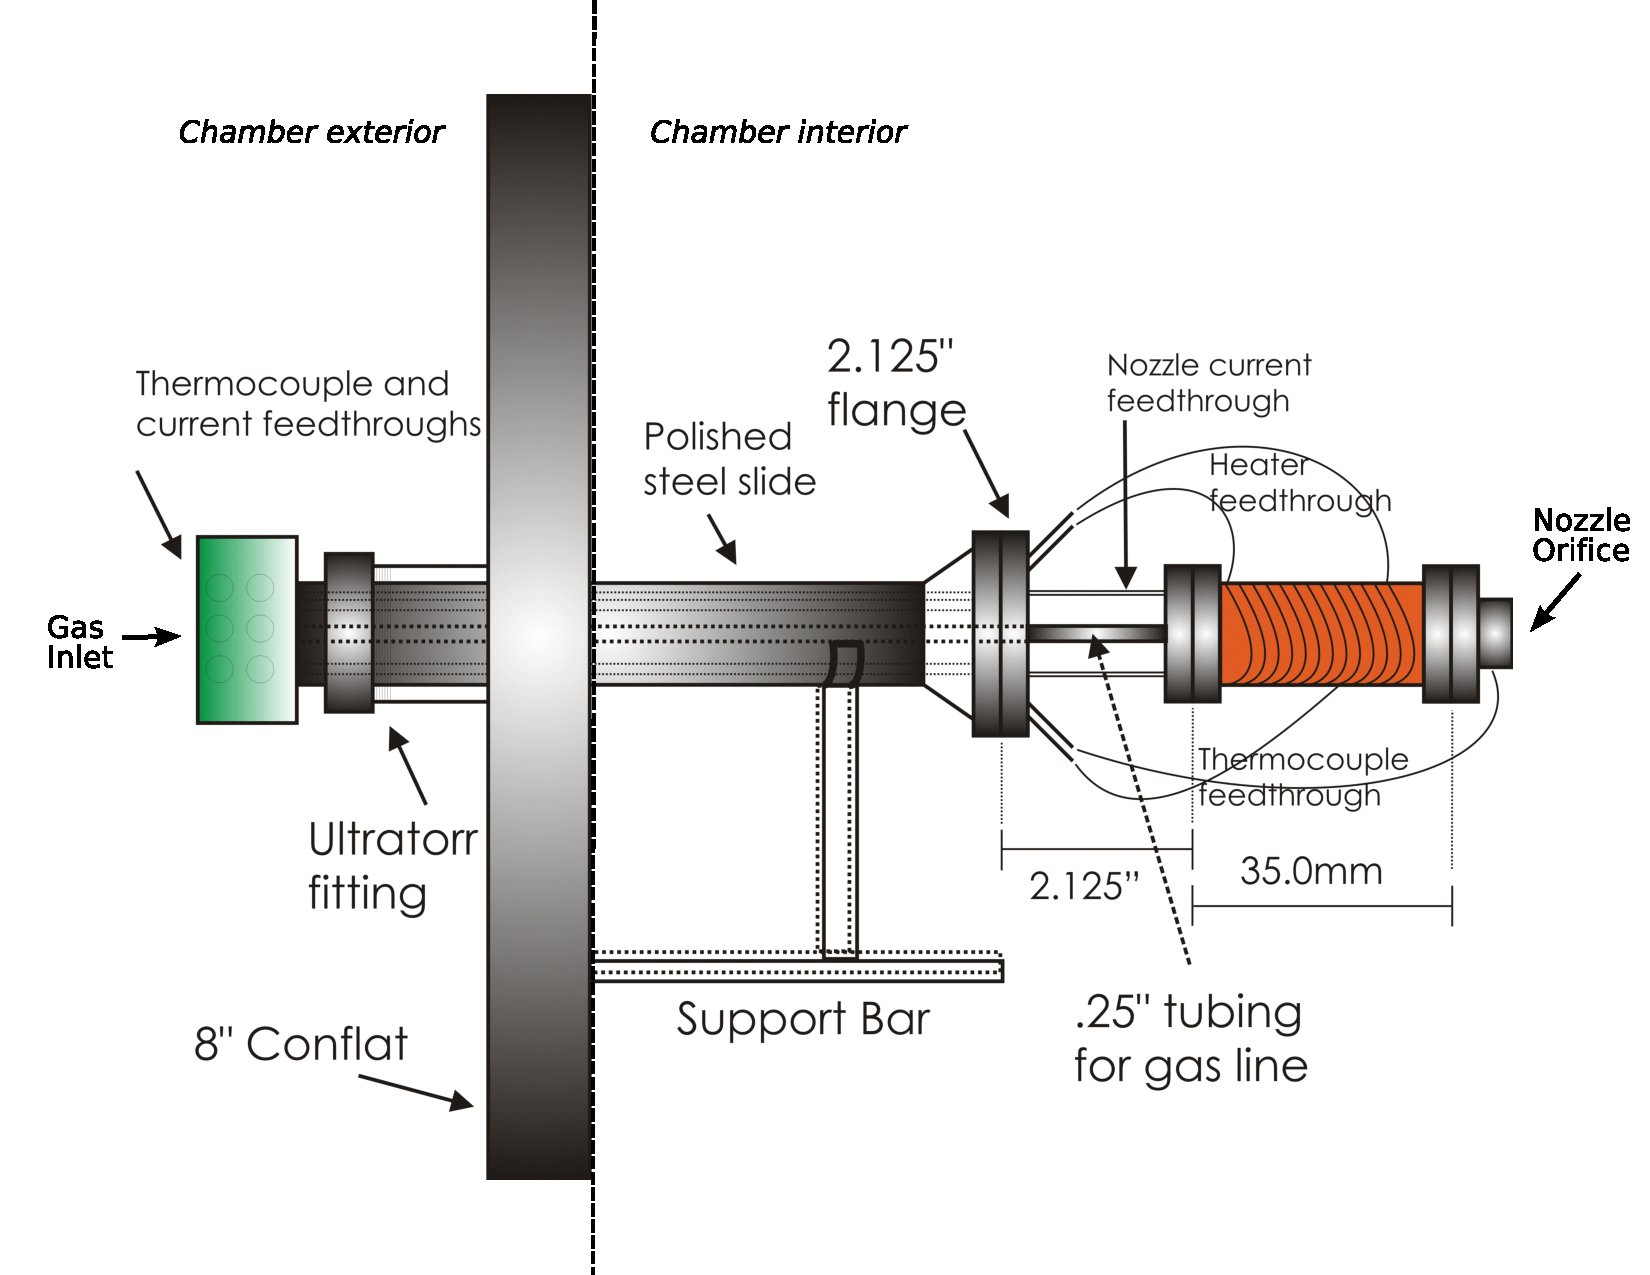
\includegraphics[width=6in]{bern-diagram.pdf}
\end{figure}

We attempted to populate the $^3P_0$ level of mercury by collisional
relaxation with \ce{N2} molecules.  Nitrogen is known to efficiently
quench Hg*($6 \; ^3P_1$) to Hg*($6 \; ^3P_0$), because the
intramultiplet energy difference is about the same as the vibrational
level spacing in \ce{N2} \cite{callear70, horiguchi71}.  Bras and
coworkers meaured the energy transfer dynamics of mercury in \ce{N2}
buffer gas, and determined that Hg($^3P_0$) may be efficiently
produced by the decay process Hg($7 \; ^1S_0$) $\rightarrow$ Hg($6 \;
^3P_1$) $\rightarrow$ Hg($6 \; ^3P_0$) \cite{bras93}.

The relatively strong one color, two-photon transition Hg $7 \; ^1S_0$
$\leftarrow\leftarrow$ $6 \; ^1S_0$ was recorded under static cell
conditions.  However, the excitation energy of Hg*($^3P_0$) is below
the work function of gold.  A Yttrium surface was tested in an effort
to develop a lower work function SEELEM detector.  As part of a
collaborative project with Trevor Sears, we installed a Yttrium
surface on our SEELEM detector and attempted to measure the signal
from metastable phenylacetylene molecules.  Following laser excitation
of several $\tilde{A}$-state vibrational levels, a TOF:SEELEM spectrum
was recorded.  TOF:SEELEM spectra are plotted for all phenylacetylene
levels measured in Figure \ref{fig:phenylacetylene-tofs}.
Unfortunately, we were not able to maintain the detector in a reliable
state of operation with a yttrium surface.  We turned to methods for
creating Hg($^3P_2$).

\begin{figure}
  \caption{TOF:SEELEM spectra of several vibrational levels of
    $\tilde{A}$ phenylacetylene.  The levels are labeled according to
    their energy above the origin band.
    }
  \label{fig:phenylacetylene-tofs}
  \centering
  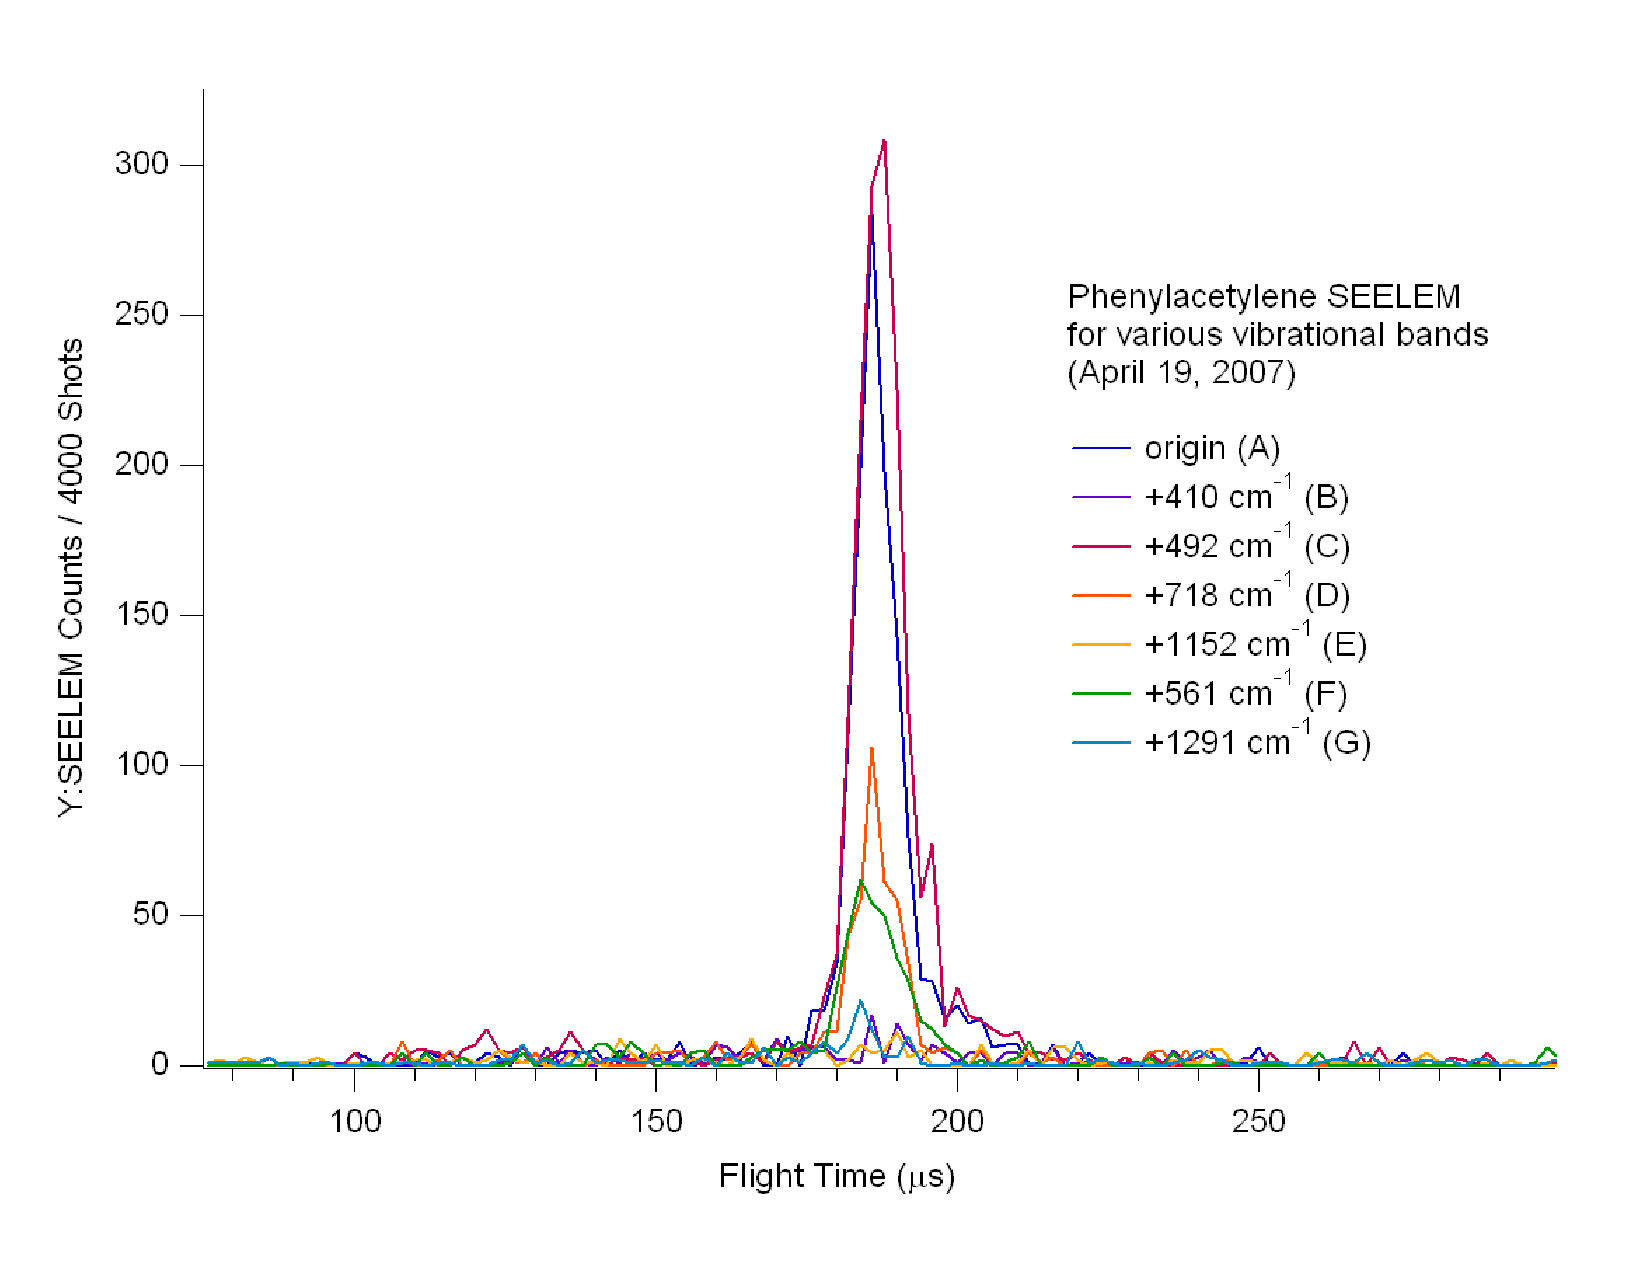
\includegraphics[width=8in,angle=90]{phenylacetylene-tofs.pdf}
\end{figure}

Following our success with xenon, we attempted to use the $6\;^3D_2
\leftarrow \leftarrow 6\;^1S_0$ one color, two-photon transition to
create mercury atoms in the $^3P_2$ state.

\begin{figure}
  \caption{Laser-Induced Fluorescence (LIF) spectrum of the one color,
    two photon transition \ce{Hg} $6\;^3D_2 \leftarrow \leftarrow
    6\;^1S_0$, recorded under static cell conditions.  The LIF signal
    results from spontaneous emission to the metastable $6\;^3P_2$
    state at 365 nm.}
  \label{fig:hg3d2-cell}
  \centering
  \vspace{1cm}
  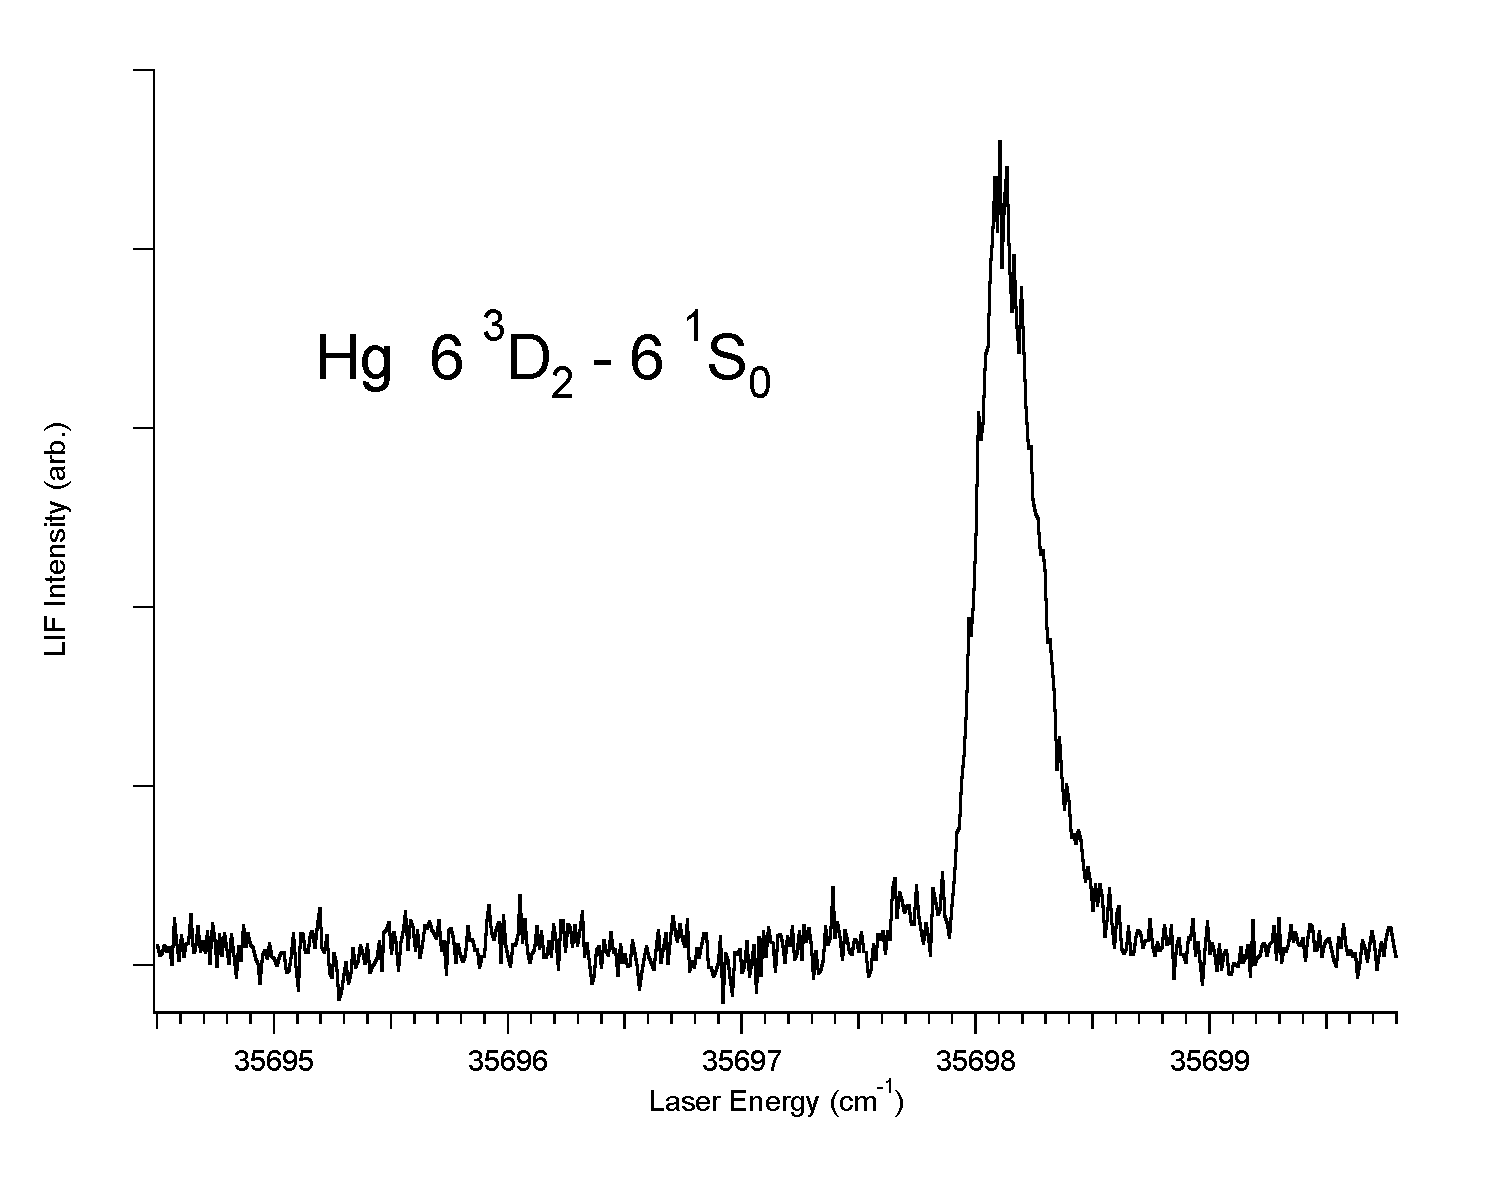
\includegraphics[width=6in]{Hg3D2-cell.pdf}
  \vspace{1cm}
\end{figure}

Direct excitation to the $^3P_2$ was also attempted as a method for
triplet formation.  This transition, while forbidden in the solitary
molecule, is made allowed in collision complexes with a variety of
gases \cite{kurosawa98, amano98}.  Also, we note that weak Hg*($6 \; ^3P_2$)
$\rightarrow$ Hg($6 \; ^1S_0$) emission was observed in pre-laser
experiments \cite{mrozowski45}.  Figure \ref{fig:hg-3p2-direct} shows
the TOF:SEELEM spectrum of mercury excited to directly to the $6 \;
^3P_2$ level.  The signal level is sufficiently low that it is checked
against a repeated experiment with the pulsed valve turned off, shown
for comparison in Figure \ref{fig:hg-3p2-direct-bg}.  While it is
clear that we do register a SEELEM signal from the direct excitation
of Hg*($6 \; ^3P_2$), we were not able to increase the gas density
enough at the excitation point to make this an efficient process for
the population of acetylene metastables.

\begin{figure}
  \caption{SEELEM time of flight (TOF) detection of metastable mercury
    produced via the direct excitation Hg*($6 \; ^3P_2$) $\leftarrow$
    Hg($6 \; ^1S_0$) at 44042.98 \rcm.  The pulsed valve was heated to
    250\degrees\ C to increase the number density of mercury.  The two
    traces are recorded in repeated experiments.}
\label{fig:hg-3p2-direct}
\centering
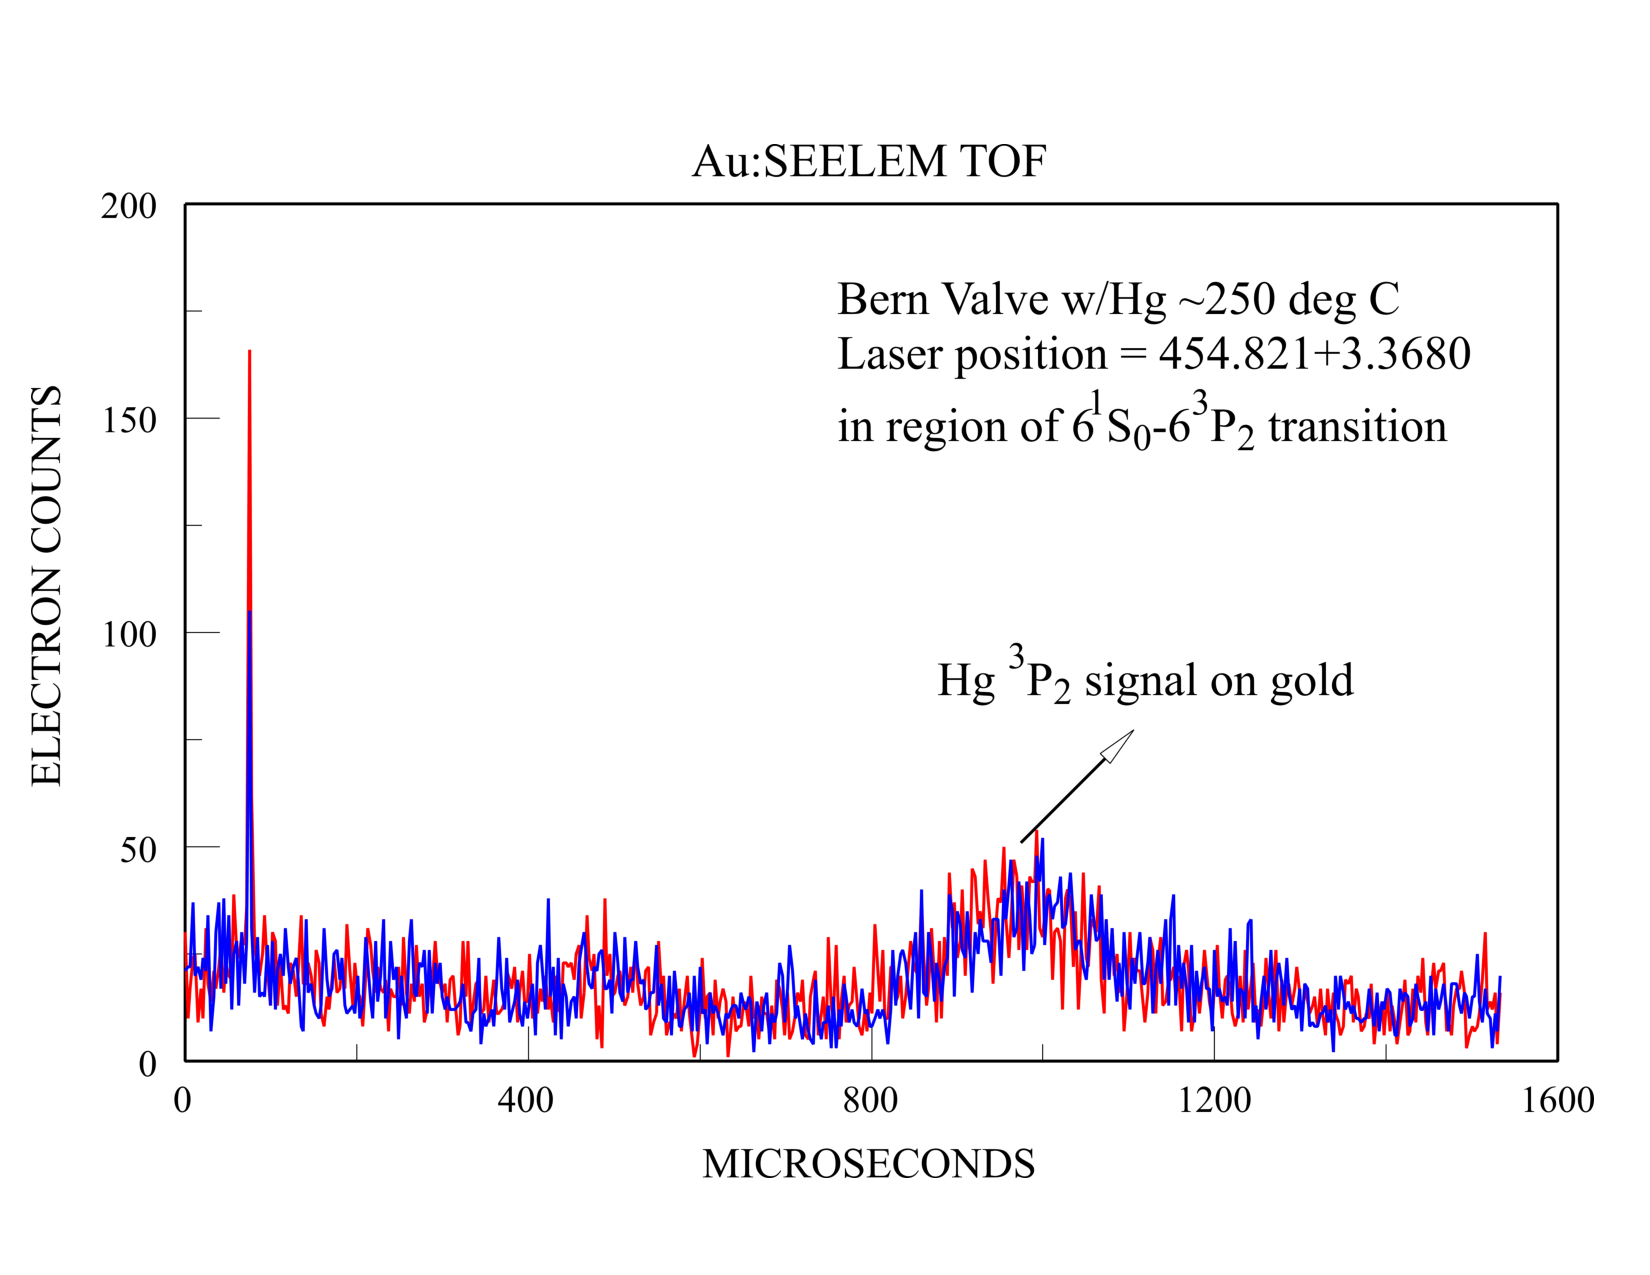
\includegraphics[width=8in,angle=90]{hg-3p2-direct.pdf}
\end{figure}

\begin{figure}
  \caption{Comparison of signal to background in the SEELEM time of
    flight (TOF) detection of metastable mercury produced via the
    direct excitation Hg*($6 \; ^3P_2$) $\leftarrow$ Hg($6 \; ^1S_0$)
    at 44042.98 \rcm.  The lighter trace is recorded with the pulsed
    valve on, and the black trace is recorded with the valve off.}
\label{fig:hg-3p2-direct-bg}
\centering
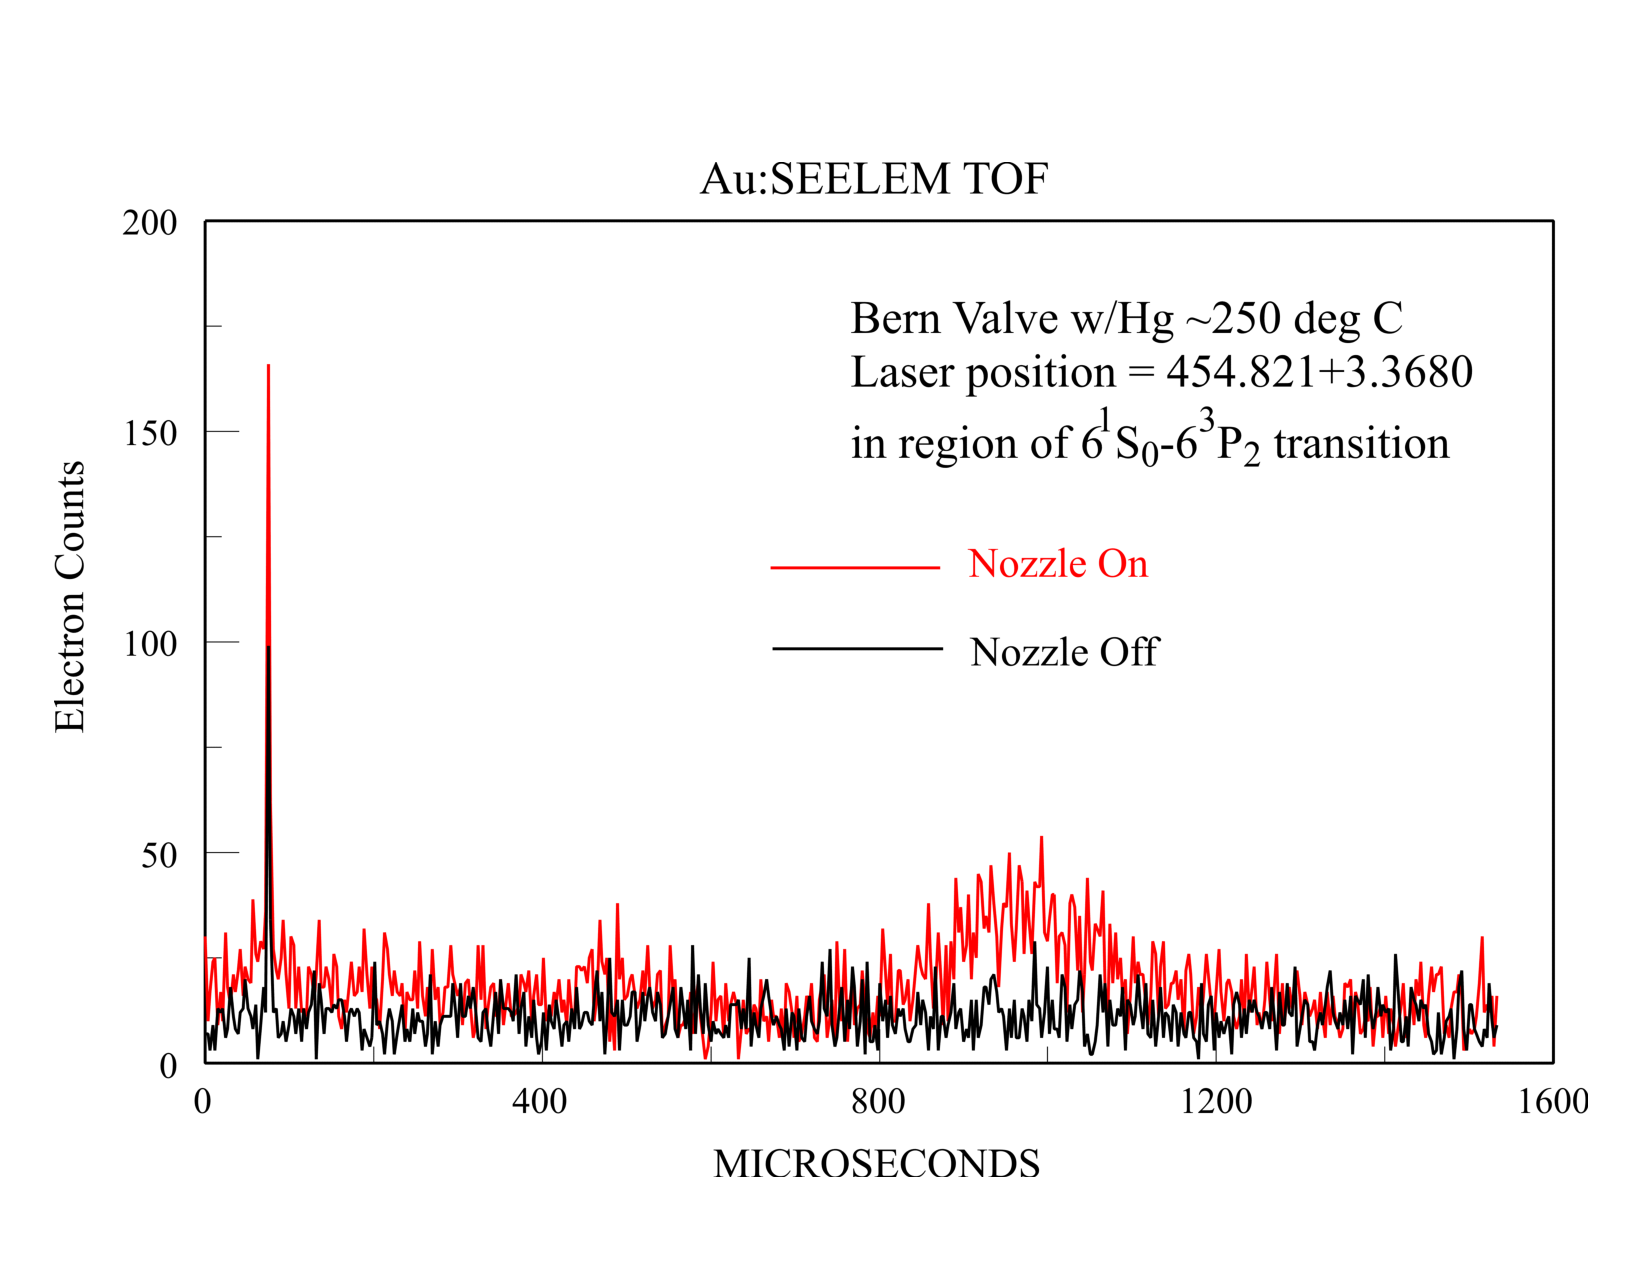
\includegraphics[width=8in,angle=90]{hg-3p2-direct-bg.pdf}
\end{figure}

The most efficient method found for the population of mercury $6 \;
^3P_2$ was a simple, two step excitation to $7 \; ^3S_1$ via the $6 \;
^3P_1$ level.  It was found that this method did not produce any
polymer when used in a pulsed supersonic expansion.  

Figure \ref{fig:hg-twostep} shows the LIF spectrum of the $6 \; ^3P_1
\leftarrow 6\;^1S_0$ transition.  The hyperfine structure of the
\ce{^{199}Hg} and \ce{^{201}Hg} isotopes is apparent in the lineshape
of the transition.

\begin{figure}
  \caption{Simultaneously recorded LIF and SEELEM spectra for the
    two-color, stepwise excitation of Hg($^3S_1$) via the $^3P_1$
    level.  An interference filter was used to record only Hg($^3S_1$)
    $\rightarrow$ Hg($^3P_2$) emission, which results in the
    population of metastable Hg atoms.  The SEELEM spectrum detects
    the metastables after a 700 \microsec\ flight time.  The structure
    in the spectrum is the result of hyperfine splittings in the odd
    isotopes of mercury, \ce{^{199}Hg} and \ce{^{201}Hg}.}
  \label{fig:hg-twostep}
  \centering
  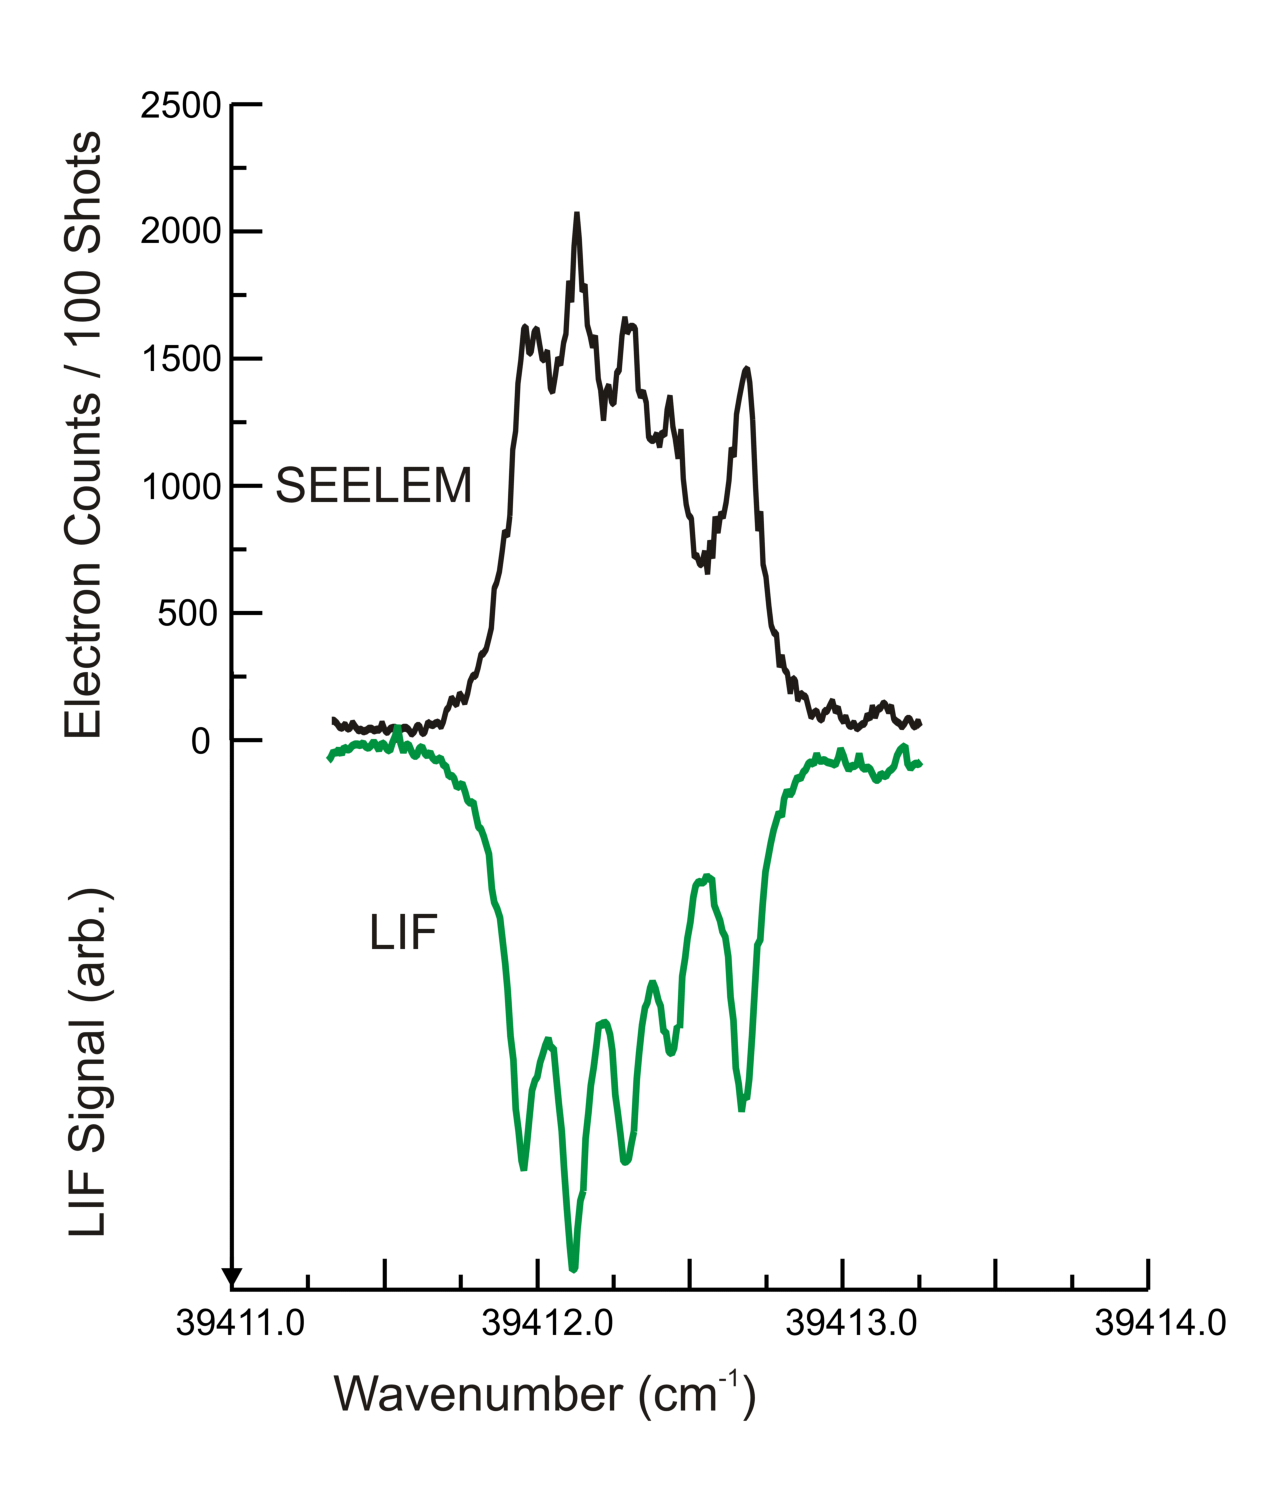
\includegraphics[width=6.5in]{hg-twostep.pdf}
\end{figure}

\begin{figure}
  \caption{SEELEM spectrum of the two-color, stepwise excitation of
    Hg($^3S_1$) via the $^3P_1$ level.  The lower spectrum shows
    mercury seeded in Xe gas, while the upper spectrum shows mercury
    seeded in acetylene.  The larger overall signal level in the
    mercury/acetylene mixture is the result of electronic excitation
    transfer between Hg($^3P_2$) and \ce{C2H2}($T_3$).}
  \label{fig:hg-twostep-c2h2}
  \centering
  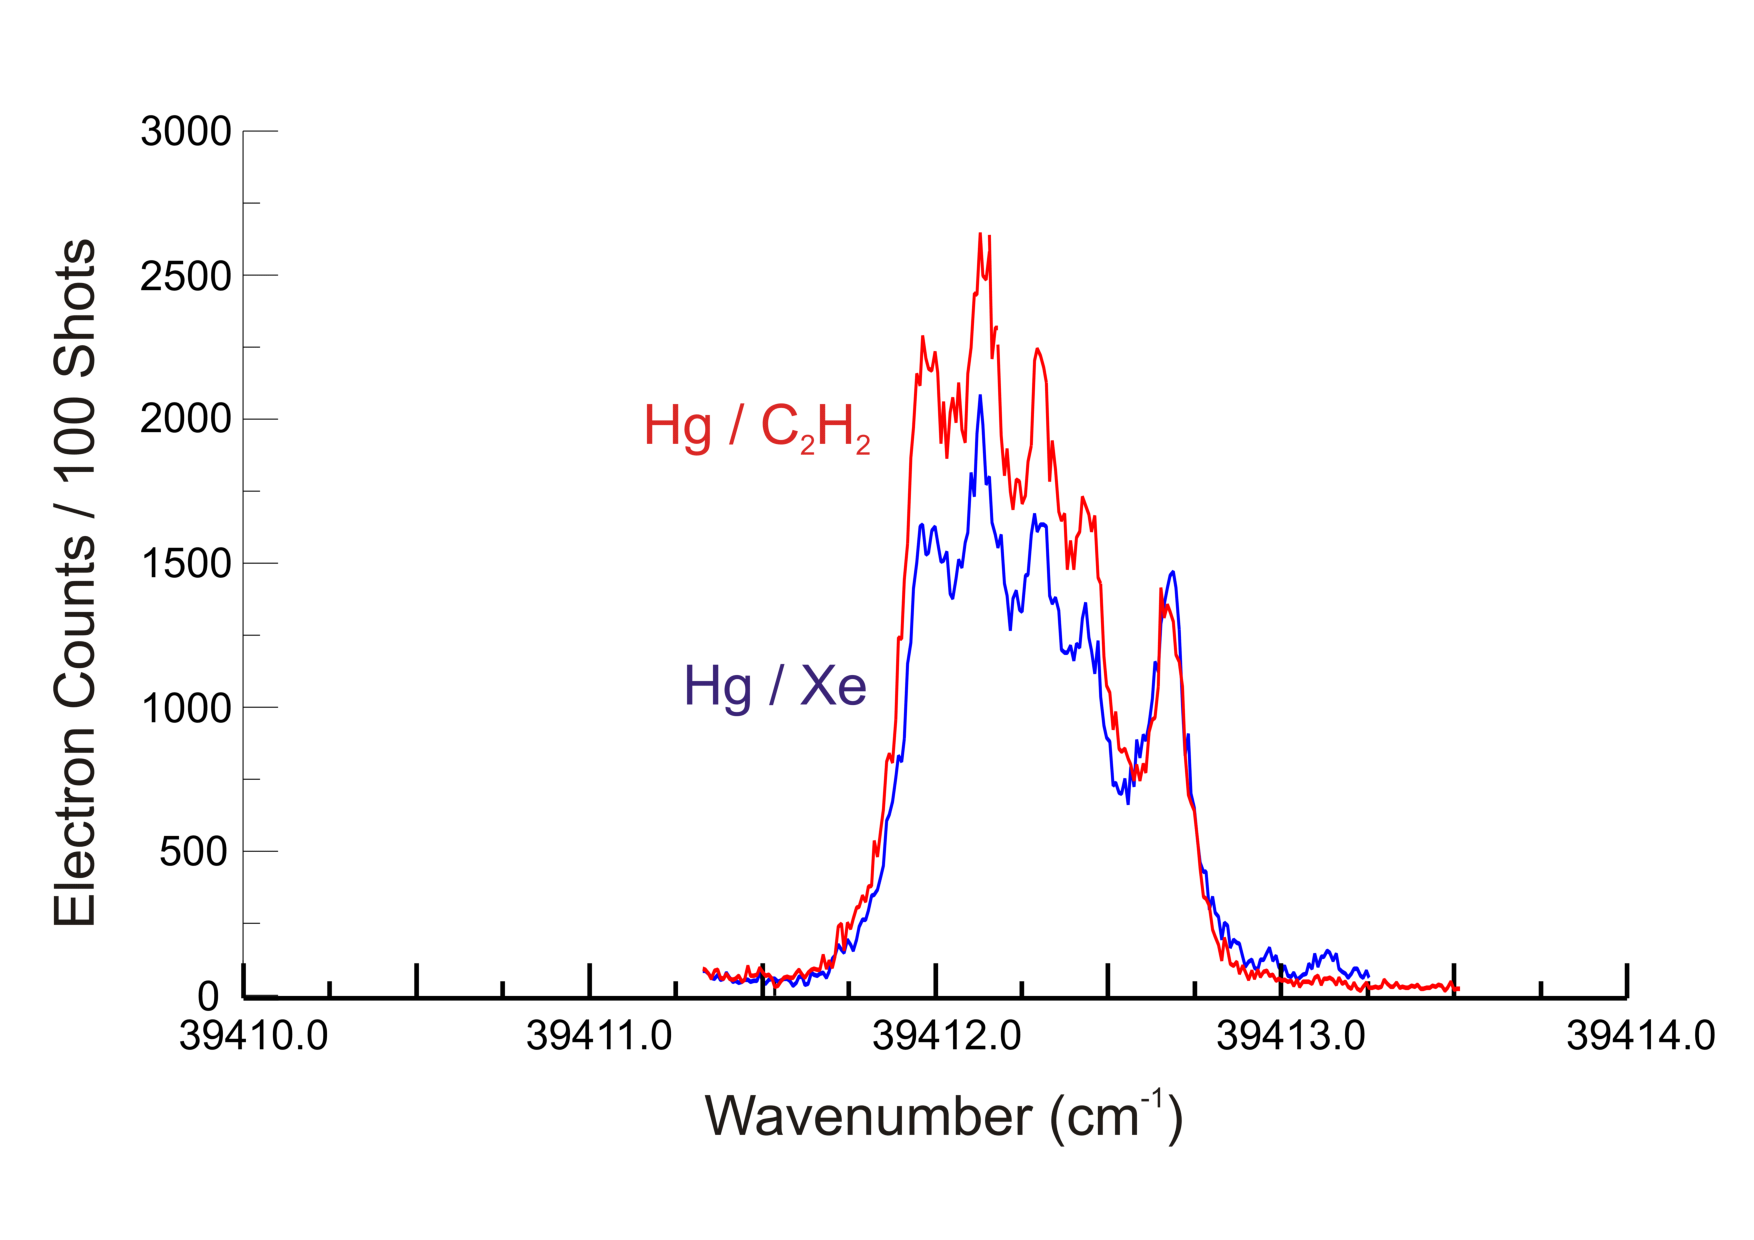
\includegraphics[width=8in,angle=90]{hg-twostep-c2h2.pdf}
\end{figure}


Methods are available to optically filter mercury resonance radiation
using mercury itself as the absorber \cite{vanzee89, senitzky74}.

\section{Future Work}

Two types of new experiments are proposed, looking at energy transfer
from atom to molecule, and vice versa.



An exciting experiment for the xenon-nitrogen system would be to study
the rotational and vibrational depenence of collision-induced reverse
intersystem crossing from the $a' \; ^1\Sigma_u^-$ state to the $B \;
^3\Pi_g$ state.  Xenon has been observed to facilitate this process,
although the rotational and vibrational dependence are uncertain
\cite{umemoto03a}.

\section{Conclusions}

We demonstrate the production of metastable acetylene and nitrogen
molecules in a molecular beam by the method of collisional electronic
excitation.  Metastable atoms, populated by two-photon transitions
followed by spontaneous emission, are used as collision partners.  A
study of the TOF:SEELEM spectrum reveals translationally exothermic
energy transfer in the Xe*($6 \; ^3P_2$) + \ce{N2} system.


\bibliography{master} 
\bibliographystyle{plain}
\end{document}